\documentclass[a4paper,12pt,oneside,onecolumn]{book}
\linespread{1.5}
\usepackage[utf8]{inputenc}                                      
\usepackage[T1]{fontenc}  
\usepackage{helvet}
\renewcommand{\familydefault}{\sfdefault}
\usepackage{amsmath,amsfonts,amssymb,amsthm}
\usepackage{csquotes}
\usepackage[margin=2.5cm]{geometry}
\usepackage{graphicx}
\usepackage{xcolor}
\usepackage{array}
\graphicspath{ {images/} } % folder z grafiką
\usepackage{url}
\usepackage{hyperref}
\usepackage{indentfirst}
% % 3 kwietnia
\usepackage[american, polish]{babel}
\usepackage[backend=biber, giveninits=false, style=apa, sorting=nyt, autolang=other, language=american, defernumbers=true]{biblatex}
% % 3 kwietnia
\usepackage{listings}
\usepackage{fancyhdr}
\usepackage{etoolbox}
\usepackage{float}
\usepackage{cprotect}
\usepackage[nottoc, notlof, notlot, numbib]{tocbibind}
\usepackage{caption}


%\patchcmd{\chapter}{\thispagestyle{plain}}{\thispagestyle{fancy}}{}{}
% color def
\usepackage{color}
\definecolor{darkred}{rgb}{0.6,0.0,0.0}
\definecolor{darkgreen}{rgb}{0,0.50,0}
\definecolor{lightblue}{rgb}{0.0,0.42,0.91}
\definecolor{orange}{rgb}{0.99,0.48,0.13}
\definecolor{grass}{rgb}{0.18,0.80,0.18}
\definecolor{pink}{rgb}{0.97,0.15,0.45}


% General Setting of listings
\lstset{
  aboveskip=1em,
  breaklines=true,
  abovecaptionskip=-6pt,
  captionpos=b,
  escapeinside={\%*}{*)},
  frame=single,
  numbers=left,
  numbersep=15pt,
  numberstyle=\tiny,
  showstringspaces=false
}
% 0. Basic Color Theme
\lstdefinestyle{colored}{ %
  basicstyle=\ttfamily,
  backgroundcolor=\color{white},
  commentstyle=\color{green}\itshape,
  keywordstyle=\color{blue}\bfseries\itshape,
  stringstyle=\color{red},
}
% 1. General Python Keywords List
\lstdefinelanguage{PythonPlus}[]{Python}{
  morekeywords=[1]{,as,assert,nonlocal,with,yield,self,True,False,None,} % Python builtin
  morekeywords=[2]{,__init__,__add__,__mul__,__div__,__sub__,__call__,__getitem__,__setitem__,__eq__,__ne__,__nonzero__,__rmul__,__radd__,__repr__,__str__,__get__,__truediv__,__pow__,__name__,__future__,__all__,}, % magic methods
  morekeywords=[3]{,object,type,isinstance,copy,deepcopy,zip,enumerate,reversed,list,set,len,dict,tuple,range,xrange,append,execfile,real,imag,reduce,str,repr,}, % common functions
  morekeywords=[4]{,Exception,NameError,IndexError,SyntaxError,TypeError,ValueError,OverflowError,ZeroDivisionError,}, % errors
  morekeywords=[5]{,ode,fsolve,sqrt,exp,sin,cos,arctan,arctan2,arccos,pi, array,norm,solve,dot,arange,isscalar,max,sum,flatten,shape,reshape,find,any,all,abs,plot,linspace,legend,quad,polyval,polyfit,hstack,concatenate,vstack,column_stack,empty,zeros,ones,rand,vander,grid,pcolor,eig,eigs,eigvals,svd,qr,tan,det,logspace,roll,min,mean,cumsum,cumprod,diff,vectorize,lstsq,cla,eye,xlabel,ylabel,squeeze,}, % numpy / math
}
% 2. New Language based on Python
\lstdefinelanguage{PyBrIM}[]{PythonPlus}{
  emph={d,E,a,Fc28,Fy,Fu,D,des,supplier,Material,Rectangle,PyElmt},
}
% 3. Extended theme
\lstdefinestyle{colorEX}{
  basicstyle=\ttfamily,
  backgroundcolor=\color{white},
  commentstyle=\color{darkgreen}\slshape,
  keywordstyle=\color{blue}\bfseries\itshape,
  keywordstyle=[2]\color{blue}\bfseries,
  keywordstyle=[3]\color{grass},
  keywordstyle=[4]\color{red},
  keywordstyle=[5]\color{orange},
  stringstyle=\color{darkred},
  emphstyle=\color{pink}\underbar,
}

\lstset{style=colorEX}
\lstset{inputpath=chapters/Code/}


% % 3 kwietnia
\DefineBibliographyStrings{american}{
  andothers = {i in., \addabbrvspace}, % Zmienia "et al." na "i in."
}
\setlength{\emergencystretch}{3em}  % allows for up to 3em of additional white space per line
\tolerance=1000 
% % 3 kwietnia

\renewcommand{\lstlistingname}{Próbka kodu}
\renewcommand{\lstlistlistingname}{Spis próbek kodu}
\renewcommand{\listfigurename}{Spis rysunków}
\renewcommand{\listtablename}{Spis tabel}
\renewcommand{\figurename}{Rysunek}
\renewcommand{\tablename}{Tabela}

\newenvironment{conditions}
  {\par\vspace{\abovedisplayskip}\noindent\begin{tabular}{>{$}l<{$} @{${}={}$} l}}
  {\end{tabular}\par\vspace{\belowdisplayskip}}

\makeatletter
\let\orgdescriptionlabel\descriptionlabel
\renewcommand*{\descriptionlabel}[1]{%
\let\orglabel\label
\let\label\@gobble
\phantomsection
\edef\@currentlabel{#1}%
%\edef\@currentlabelname{#1}%
\let\label\orglabel
\orgdescriptionlabel{#1}%
}
\makeatother

\DeclareFieldFormat{labelnumberwidth}{#1\adddot\hspace{2mm}}
\setlength{\biblabelsep}{\labelsep}

% Dodanie numeracji do każdego wpisu w bibliografii z dodatkową spacją
\DeclareFieldFormat{labelnumber}{#1\adddot}
\renewbibmacro*{begentry}{%
  \printfield{labelnumber}%
  \hspace{2mm}% Dodatkowa przestrzeń po numerze
}

% Definicje stylu dla podpisów
\captionsetup[figure]{
  font=small, % Wielkość czcionki dla podpisów
  labelfont=bf, % Pogrubione oznaczenie numeru rysunku
  justification=raggedright, % Wyrównanie tekstu podpisu do lewej
  labelsep=period, % Dodanie kropki po numerze rysunku
  singlelinecheck=off % Wymuszenie wyrównania do lewej niezależnie od długości tekstu
}

\captionsetup[lstlisting]{
  font=small, % Wielkość czcionki dla podpisów
  labelfont=bf, % Pogrubione oznaczenie numeru rysunku
  justification=raggedright, % Wyrównanie tekstu podpisu do lewej
  labelsep=period, % Dodanie kropki po numerze rysunku
  singlelinecheck=off % Wymuszenie wyrównania do lewej niezależnie od długości tekstu
}


% Ustawienia dotyczące samych rysunków
\makeatletter
\renewcommand{\fnum@figure}{Rysunek \thefigure}
\makeatother

\setlength{\abovecaptionskip}{10pt} % Odstęp nad podpisem
\setlength{\belowcaptionskip}{5pt} % Odstęp pod podpisem
\newcommand{\refnote}[1]{%
  \ref{#1}\footnote{Sekcja \ref{#1}, strona \pageref{#1}}%
}
\newcommand{\parrefnote}[1]{%
  \ref{#1}\footnote{Paragraf \ref{#1}, strona \pageref{#1}}%
}
\newcommand{\figrefnote}[1]{%
  \ref{#1}\footnote{Rysunek \ref{#1}, strona \pageref{#1}}%
}
\newcommand{\pagerefnote}[1]{%
  \pageref{#1}\footnote{Strona \pageref{#1}}%
}

\addbibresource{refs.bib}

\begin{document}

% *************** Front matter ***************
% *************** Strona tytułowa ***************

\pagestyle{empty}
\noindent
\begin{center}
    UNIWERSYTET EKONOMICZNY W KATOWICACH
\end{center}

\begin{center}
    INFORMATYKA
\end{center}

\vfill
\begin{center}
    \textbf{Jakub Stokowski}
    \par \normalsize \textbf{147719}
\end{center}
\vfill

\begin{center}
    \Large
	\textbf{Optymalizacja zespołów projektowych w firmie IT z wykorzystaniem modelu optymalizacyjnego}
\end{center}

\begin{center}
	\textbf{Optimizing project teams in an IT company using an optimization model}
\end{center}

\vfill
\vfill
\vfill

\begin{flushright}
Praca licencjacka \\
napisana w Katedrze Informatyki \\ 
pod kierunkiem dr Sławomira Jarka
\end{flushright}

\vfill
\begin{center}
    KATOWICE 2024
\end{center}

\newpage 
\pagestyle{fancy}
\fancyhf{}
\fancyhf{} % sets both header and footer to nothing
\renewcommand{\headrulewidth}{0pt}
\fancyfoot[R]{\thepage}
\newpage
\tableofcontents

% *************** Koniec front matter ***************


\clearpage
\addcontentsline{toc}{chapter}{Wprowadzenie}
\chapter*{Wprowadzenie}

\par W erze cyfrowej, gdzie technologia ewoluuje w zawrotnym tempie, każdy projekt IT staje się coraz bardziej złożony i wielowymiarowy. Zarządzanie zasobami ludzkimi w branży IT jest skomplikowane, podobnie jak kody, które programiści piszą każdego dnia. W tym dynamicznym kontekście pojawia się pytanie: jak efektywnie zarządzać takimi zespołami, aby osiągnąć sukces przy optymalnym użyciu zasobów? Odpowiedź na to pytanie nie jest prosta, ale znalezienie odpowiedzi za pomocą optymalizacji matematycznej oraz modelu optymalizacyjnego już tak.

\par Każdy projekt IT jest unikatową mozaiką zadań, technologii, oczekiwań i ludzi. Według Thomasa Keen'a \parencite{keen2003creating} "\textit{W obecnych czasach liderzy zespołów stają przed coraz to nowymi wyzwaniami ciągle zmieniającego się świata; Niestabilność rynków wymusza podejmowanie szybkich kluczowych decyzji; olbrzymie fuzje i przejęcia; wyrafinowanie klientów oraz ciągłe rotacje i niepokój wśród pracowników}". W tym labiryncie zmiennych, menedżerowie projektów stają przed trudnym zadaniem zbudowania zespołu, który nie tylko posiada odpowiednie umiejętności techniczne, ale także potrafi efektywnie współpracować, komunikować się i wprowadzać innowacje. Wyzwanie to staje się szczególnie istotne w czasach, gdy rynek IT jest nasycony, a konkurencja stale rośnie. 

\par\label{par:hipotezy} Nasuwają się dwie hipotezy, pierwsza (H1) - czy jest możliwe stworzenie modelu matematycznego, który będzie w stanie stworzyć optymalny zespół pracowników dla zadanych ograniczeń. Drugą hipotezą (H2) jest kwestia implementacji owego modelu - czy implementacja takiego modelu i jego analiza może zostać przeprowadzona w języku programowania w Python? Na te dwa pytania praca postara się uzyskać odpowiedź poprzez analizę literatury przedmiotu, studium przypadku oraz analizę wyników modelu.

\par Celem tej pracy jest opracowanie oraz implementacje takiego modelu optymalizacyjnego, który będzie w stanie wybrać optymalny zespół pracowników, spełniając wszystkie założone wymagania. Poprzez zastosowanie solidnych podstaw teoretycznych oraz przeprowadzenie praktycznych eksperymentów, praca ta chce dopowiedzieć na kluczowe pytanie: jak matematyczna precyzja może przekształcić chaos zarządzania projektami w dobrze funkcjonujący mechanizm. Jak twierdzi Al-mosa i in. w ostatnich latach, modelowanie matematyczne pełniło kluczową rolę w wielu sektorach życia. Od informatyki, przez fizykę i chemię aż do genetyki. \parencite{almosa2023python}.

\par W obliczu ciągle zmieniającego się świata IT i rosnącej konkurencji, utworzenie dobrze dobranego zespołu jest kluczowe dla sukcesu. Wedle Sweem S. \parencite{sweem2009leveraging}, w firmach utrzymujących się na rynku ciągle zachodzą zmiany. Jest to stale powodowane strategiami zarządzania talentów. Tezę te potwierdzają również autorzy \parencite{rusilowati2024optimizing}. Wedle przeprowadzonego przez autorów badania, w obecnie szybko rozwijającym się świecie, planowanie zasobów ludzkich stało się kluczowe dla organizacji. Stwierdza również, że dla wielu firm optymalizacja procesów (z zakresu zrządzania zespołami) nadal stanowi wyzwanie. Można z tego wywnioskować, że często zachodząca rotacja talentów w firmie może utrudniać ciągłe wybieranie nowych zespołów i znajdywanie tzw. "złotego środka". Jak twierdzi Ashcraft \parencite{ashcraft2011ipd}, zespoły dostarczają właściwej wiedzy we właściwym czasie, pobudzają kreatywność i obniżają bariery między uczestnikami projektu. Dodatkowo, procesy zespołowe usprawniają podejmowanie decyzji, a wspólne wybory zwiększają poparcie dla wybranych strategii. Niezwykle ważnym jest więc optymalne utworzenie zespołu, który będzie stać na wysokości zadania dla zapewnienia sukcesu projektu, w odpowiednio krótkim czasie.

\par W kontekście modelu optymalizacyjnego zaprezentowanego w tej pracy, celem jest minimalizacja całkowitego kosztu zatrudnienia pracowników przy jednoczesnym zapewnieniu, że zespół posiada niezbędne umiejętności techniczne kluczowe dla ukończenia projektu. Według Aithala'a \parencite{aithal2016theory}, optymalizacja wydajności jest trudnym procesem dla firmy, który wymaga wydobycia najwyższej produktywności z pracowników, przy utrzymaniu ograniczeń organizacyjnych. Celem pracy jest ułatwienie tego procesu za pomocą modelu optymalizacyjnego. Wspomniane ograniczenia zostaną zawarte w modelu, a ten wybierze optymalny zespół, nie przekraczając ich.

\par Zastosowanie takiego modelu w organizacjach IT, może przynieść wymierne korzyści. Według Wei \parencite{wei2022optimal}, optymalizacja zasobów ludzkich polega na umieszczeniu odpowiednich ludzi, w odpowiednim miejscu w celu maksymalizacji ich wartości. Zastosowanie proponowanego modelu optymalizacyjnego może pomóc menedżerom dokonać właśnie tego. Dodatkowo pozwoli na lepsze zrozumienie, jak różne kombinacje umiejętności i kompetencji wpływają na wydajność projektu, co w efekcie prowadzi do bardziej świadomego i efektywnego zarządzania zasobami ludzkimi. Zarządzanie zasobami ludzkimi (HR) jest właśnie tym według autora \parencite{albi2024innovative}. Autor stwierdza, że HR jest domeną skupiającą się szczególnie na interakcjach i funkcjach osób w organizacji. Dotyczy to również optymalnego wykorzystania tych osób do osiągnięcia optymalnego poziomu wydajności i skuteczności w osiąganiu celów firmy. 

\par Ponadto, cel pracy obejmuje analizę literatury przedmiotu oraz przeprowadzenie badań, które mają na celu potwierdzenie skuteczności zaproponowanego modelu. Istotnym aspektem tej analizy jest zidentyfikowanie najlepszych praktyk w zakresie optymalizacji zasobów ludzkich oraz zrozumienie czym jest produktywność jednostki i co na nią wpływa. Hermawan określa produktywność pracowników jako wynik pracy osoby w określonym czasie, na określonej ilości zadań i ze spełnioną ilością celów \parencite{hermawan2020optimizing}. Natomiast Syverson \parencite{syverson2011determines} określa produktywność jako różnice między wykorzystanymi zasobami, a uzyskanym produktem przez firmę.

\par Kolejnym celem jest opracowanie narzędzia, które będzie łatwe w implementacji i użytkowaniu przez menedżerów projektów lub dział kadr (HR) w firmach IT. Model optymalizacyjny zaprojektowany w tej pracy ma być wsparciem w codziennych decyzjach menedżerskich, umożliwiając szybkie i efektywne tworzenie zespołów projektowych dostosowanych do specyficznych wymagań projektów. Dział HR, jak twierdzi autor \parencite{sihombing2024optimizing}, ogrywa ważną rolę w optymalizacji wydajności współpracy w firmie oraz napędza sukcesy organizacji. Spowodowane jest to, jak twierdzi Larson E. \parencite{larson2014project}, "\textit{ Wzrost gospodarczy jest osiągany przez nowe miejsca pracy i przewagę konkurencyjną, które są efektem ciągłej innowacji, opracowywania nowych produktów i usług oraz poprawy zarówno produktywności, jak i jakości pracy. To jest świat zarządzania projektami.}".

\par Implementacja modelu za pomocą technik programowania liniowego za pomocą języka Python i bibliotek takich jak \verb|PuLP|, ma na celu pokazanie praktycznych aspektów jego zastosowania. Wedle Mitchelle'a \parencite{mitchell2009introduction} użycie biblioteki \verb|PuLP| do modelowania i rozwiązywanie problemów optymalizacyjnych może być bardzo wygodnym podejściem dla programisty Python'a. Użycie tego pakietu pozwala skupić się na samym modelowaniu, bez potrzeby wymyślania i implementowania algorytmu do jego rozwiązania. Solvery używane przez \verb|PuLP| to dojrzałe oprogramowania, którym można powierzyć wybór odpowiednio algorytmu do optymalizacji. 



\par Podsumowując, celem niniejszej pracy jest nie tylko teoretyczne opracowanie modelu optymalizacyjnego, ale również kwestia jego praktycznego zastosowania w rzeczywistych scenariuszach zarządzania zespołami. Dostarczenie narzędzia, które wspiera menedżerów w podejmowaniu bardziej świadomych i efektywnych decyzji przy tworzeniu zespołów jest ważnym punktem tej pracy. 


\chapter{Podstawy teoretyczne}
\par W tym rozdziale zostaną omówione kluczowe aspekty podstaw teoretycznych programowania liniowego (LP) i skutecznego zarządzania zasobami ludzkimi. Wymienione również będą zastosowania LP oraz korzyści płynące z dobrego zarządzania kadrami. Według George'a B. Dantzig'a - twórcy LP - "\textit{programowanie liniowe można postrzegać jako część wielkiego rozwój, jaki dał ludzkości umiejętność formułowania ogólnych celów i wyznaczania ścieżki ich osiągnięcia poprzez szczegółowe decyzje, które należy podjąć, aby „najlepiej” osiągnąć swoje cele w obliczu praktycznych sytuacji o dużej złożoności.}" \parencite{dantzig2002linear}.

\section{Programowanie liniowe - definicja}
\par Programowanie liniowe (LP, od ang. Linear Programming) jest metodą matematyczną stosowaną do optymalizacji rozmieszczenia ograniczonych zasobów w celu osiągnięcia określonego celu. LP znajduje szerokie zastosowanie w różnych dziedzinach, od zarządzania operacyjnego po inżynierię i ekonomię. Tezę te potwierdza Paraganiha K. \parencite{parganiha2018linear} tłumacząc, że LP nie jest nową nauką i jest użyteczne dla każdej organizacji, której zależy na maksymalizacji przychodów: "\textit{Chociaż wiele organizacji biznesowych widzi programowanie liniowe jako nowa nauka lub najnowsze osiągnięcie w historii matematyki, nie ma nic nowego w maksymalizacji zysku w dowolnej organizacji biznesowej.}"
    
\par Definicję programowania liniowego przedstawia Mitchell S. \parencite{pratomoatmojo2020brief}, mówiącą że LP jest techniką tworzącą model, który może zostać użyty do rozwiązania problemu przydzielania zasobów przy założonych ograniczeniach. Mówiąc szerzej, LP to metoda optymalizacji, która pozwala na znajdowanie najlepszego rozwiązania z danego zestawu możliwości, opierając się na matematycznej reprezentacji problemu. W ramach tej metody zarówno funkcja celu, którą należy zminimalizować lub zmaksymalizować, jak i ograniczenia, które definiują dopuszczalne rozwiązania, są przedstawiane za pomocą równań liniowych. Funkcja celu w programowaniu liniowym jest wyrażona jako liniowa kombinacja zmiennych decyzyjnych i może wyglądać w ten sposób: 

\[
X = \{ x \in \mathbb{R}^n : Ax = b, x > 0 \}
\]
\[
\min z = \langle c, x \rangle
\]

gdzie:
\begin{itemize}
    \item \( X \) oznacza zbiór wszystkich wektorów \( x \) spełniających podane warunki, gdzie każdy wektor \( x \) musi należeć do przestrzeni \( \mathbb{R}^n \) i być dodatni (\( x > 0 \)).
    \item \( Ax = b \) oznacza system liniowych równań, gdzie \( A \) jest macierzą o wymiarach \( m \times n \), a \( b \) jest wektorem o \( m \) składowych, definiującym wartości po prawej stronie równań.
    \item \( x > 0 \) wskazuje, że wszystkie elementy wektora \( x \) muszą być większe od zera.
    \item \( \min z = \langle c, x \rangle \) definiuje funkcję celu, która ma być zminimalizowana. Może zostać zamienione na \( \max z = \langle c, x \rangle \)\( z \) jest wartością funkcji celu, a \( \langle c, x \rangle \) reprezentuje iloczyn skalarny wektora współczynników \( c \) i wektora zmiennych \( x \), określający wkład każdej zmiennej do wartości funkcji celu.
\end{itemize}

\par Ograniczenia w programowaniu liniowym określają warunki, które muszą być spełnione przez zmienne decyzyjne. Te ograniczenia są również przedstawiane za pomocą równań lub nierówności liniowych. Mogą one dotyczyć na przykład limitów zasobów, wymagań produkcyjnych, bądź innych technicznych lub finansowych aspektów problemu. Przykładowe ograniczenie:

\[
\sum_{j=1}^{n} A_{ij} x_j \leq b_i
\]

gdzie:
\begin{itemize}
    \item \( \sum_{j=1}^{n} A_{ij} x_j \) oznacza sumę ważoną zmiennych \( x_j \), gdzie \( j \) jest indeksem biegnącym od 1 do \( n \). Każda zmienna \( x_j \) jest pomnożona przez odpowiadający jej współczynnik \( A_{ij} \) z i-tego wiersza macierzy \( A \).
    \item \( \leq b_i \) oznacza, że wartość tej sumy ważonej nie może przekroczyć \( b_i \), co jest ograniczeniem określonym przez wartość \( b_i \) dla i-tego wiersza. 
\end{itemize}
    
\section{Algorytmy w programowaniu liniowym}
\par Do rozwiązywania problemów programowania liniowego wykorzystuje się różne algorytmy, najbardziej znanym jest metoda Simpleks opracowana przez George'a Dantziga. Jak twierdzi sam autor "\textit{metoda simplex, która przekształca raczej niewyrafinowany model LP ekonomii w podstawowe narzędzie do praktycznego planowania dużych, złożonych systemów}" \parencite{dantzig2002linear}. Algorytmy te eksplorują możliwe rozwiązania w poszukiwaniu tego, które najlepiej spełnia funkcję celu przy jednoczesnym przestrzeganiu wszystkich ograniczeń. W praktyce oznacza to znajdowanie punktów na przecięciu ograniczeń, które dają optymalne wartości dla funkcji celu. Do innych metod rozwiązywania problemów LP należą metoda geometryczna opisana na przykładzie przez Wierciak Ewę i Bugajskiego Arkadiusza w \parencite{BibEntry2024Jun}.
    

    
%\par Zarządzanie zasobami ludzkimi w kontekście projektów IT odgrywa kluczową rolę w osiąganiu celów projektowych. Zarządzanie zasobami ludzkimi obejmuje procesy organizowania, zarządzania i prowadzenia zespołu projektowego. Wchodzą w to aspekty kulturowe, poziom umiejętności, doświadczenie oraz umiejętności interpersonalne członków zespołu. 
%\par Efektywne zarządzanie zespołami projektowymi wymaga rozległej wiedzy i kompetencji w zakresie zarządzania ludźmi. Zarządzanie projektami wymaga nie tylko wiedzy technicznej, ale również umiejętności interpersonalnych i zdolności zarządzania zasobami ludzkimi. Współczesne podejście do zarządzania zasobami ludzkimi w projektach obejmuje aspekty takie jak motywowanie, komunikacja, przywództwo i rozwiązywanie konfliktów.
%\par W branży IT, zarządzanie zasobami ludzkimi napotyka na specyficzne wyzwania, takie jak szybka zmiana technologii, wysoki poziom specjalizacji oraz potrzeba ciągłego rozwoju i adaptacji pracowników. W branży IT wiedza i umiejętności, dzięki szybkiemu rozwojowi dziedziny, szybko tracą ważność, stąd konieczność ciągłego uczenia się i rozwoju, aby dalej pozostać konkurencyjnym na rynku pracy.
%\par Najlepsze praktyki w zarządzaniu zespołami projektowymi w IT obejmują: elastyczność w zarządzaniu, promowanie kultury ciągłego uczenia się, efektywne komunikowanie się i jasne określenie oczekiwań. Zarządzanie zasobami ludzkimi w zespołach projektowych IT jest złożonym procesem, wymagającym równoważenia różnych umiejętności i potrzeb. Optymalizacja składu zespołu projektowego, z wykorzystaniem metodyk takich jak programowanie liniowe, może przyczynić się do zwiększenia efektywności zespołu projektowego, bardziej wydajnego zarządzania zespołem i sprawniejszego osiągnięcia jego celów.


\section{Istota i znaczenie efektywnego składania zespołów}
\par Składanie efektywnych zespołów projektowych jest kluczowym elementem sukcesu w zarządzaniu projektami, szczególnie w dynamicznej branży IT. Efektywne zespoły charakteryzują się nie tylko odpowiednimi umiejętnościami technicznymi, ale także zdolnością do współpracy, innowacji i efektywnej komunikacji. Kluczem jest stworzenie środowiska, w którym indywidualne talenty mogą być skutecznie połączone, a ich umiejętności w pełni wykorzystane. Według Keen T. R. \parencite{keen2003creating}, fundamentalnymi składowymi zespołu są: efektywność, współzależność, zaangażowanie i odpowiedzialność grupy. Członkowie zespołu muszą mieć wspólny końcowy cel, żeby współpracować i w celu ukierunkowania wysiłków.
\par Skład zespołu ma bezpośredni wpływ na jego wydajność i sukces projektu. Dobór odpowiednich ludzi na odpowiednie stanowiska jest jednym z najważniejszych decyzji, jakie podejmuje menedżer projektu. Według Mealiea i in. \parencite{mealiea2005strategic} menedżer ogrywa kluczową rolę w utrzymaniu atmosfery w zespole poprzez swoje codzienne aktywności. Zróżnicowanie umiejętności, doświadczenia i perspektyw może znacznie wzbogacić zespół i przyczynić się do lepszych wyników. Thomas R. Keen wspomina w swojej książce, że przed rozpoczęciem pracy muszą zostać określone 3 kluczowe aspekty: misja zespołu - dlaczego zespół istnieje, cele zespołu - co zespół próbuje osiągnąć oraz wytyczne zespołu - co określa sukces, bądź niepowodzenie szespołu \parencite{keen2003creating}.
\par Synergia w zespołach projektowych oznacza, że całkowity efekt ich współpracy jest większy niż suma poszczególnych wkładów. Ta synergia jest szczególnie ważna w projektach IT, gdzie innowacyjność i kreatywność odgrywają kluczową rolę. Katzenbach i in. \parencite{katzenbach2015wisdom} podkreślają, że zespoły zawsze działają lepiej niż jednostki. W jakiejkolwiek sytuacji wymagającej szerokiego spektrum umiejętności, zespoły zawsze przewyższają nad jednostkami.
\par Efektywne składanie zespołów projektowych w branży IT jest procesem złożonym, wymagającym nie tylko odpowiedniego doboru umiejętności, ale także budowania kultury współpracy i wzajemnego wsparcia. Odpowiedni skład zespołu, wspierany przez skuteczne przywództwo, jest fundamentem do osiągnięcia synergii i sukcesu

\section{Zastosowanie programowania liniowego}
\par Programowanie liniowe znajduje zastosowanie w wielu prężnych dziedzinach nauki, przemysłu i infrastruktury. Możliwość opisywania złożonych problemów alokacji zasobów w prosty sposób spowodowała szeroką adaptację LP, przy stawianiu czoła takim problemom. Głównymi dziedzinami, gdzie LP znajduje swoje zastosowanie są:
\begin{description}
    \item[Informatyka] Olbrzymie zbiory danych stwarzają problem nawet dla najlepszych organizacji analitycznych na świecie. Przewidywanie trendów na giełdach i rynkach świata, jest niezwykle ważne w znajdywaniu kluczowych informacji dla generowania przyszłych zysków firmy. \parencite{khandelwal2019building}
    \item[Przemysł] Wykorzystanie LP w procesie alokacji zasobów w przemyśle, może znacznie wpłynąć na zyski firmy, która sięgnie po takie rozwiązanie. Według Khandelwal'a planowanie alokacji zasobów jest ważne dla przemysłu produkcyjnego, gdyż optymalne wykorzystanie zasobów zwiększa zyski firmy \parencite{khandelwal2019building}.
    \item[Transport] Priorytetami w przemyśle transportowym są planowanie wysyłek, pasażerów i dostarczanie ich na czas. Linie lotnicze stosują techniki LP poprzez ustalanie kosztów i popytu jako czynników dla maksymalizacji zysków \parencite{khandelwal2019building}. Pokazuje to, że LP jest szeroko stosowaną techniką, gdy w grę wchodzi maksymalizacja lub minimalizacja zysków albo kosztów. 
    \item[Przemysł energetyczny] LP w przemyśle energetycznym pozwala na optymalizacje zużycia surowców używanych do produkcji oraz dystrybucji wyprodukowanej energii. Według Khandelwal'a zastosowanie LP pozwala na efektywną przebudowę sieci energetycznych \parencite{khandelwal2019building}.
\end{description}

\par Z tych twierdzeń można wyciągnąć wniosek, że LP znajduj zastosowanie tam, gdzie liczy się zysk i przestrzeganie określonych ograniczeń. Jak zauważają Katzenbach i in. \parencite{katzenbach2015wisdom} większość menedżerów zauważa wartość w zespołach, ale problemy stwarzają dopiero trudne warunki, wymagania czasowe i niewarunkowane założenia. Z tego powodu, użycie LP w zarządzaniu zasobami ludzkimi, przyniesie równie dobre efekty. Stawką utworzenia optymalnego zespołu są straty organizacji, ale zastosowanie modelu optymalizacyjnego jest w stanie szybko i efektywnie rozwiązać problem tworzenia optymalnego zespołu.
\chapter{Metodologia badań}
\par W kontekście badań nad optymalizacją zespołów projektowych, niezwykle istotne jest zrozumienie oraz zastosowanie odpowiedniej metodologii. Metodologia ta bazuje na modelu optymalizacyjnym, który umożliwia analizę i dobór najbardziej efektywnego składu zespołu w oparciu o zdefiniowane kryteria i ograniczenia. 
\par Głównym celem modelu optymalizacyjnego omawianego w pracy jest minimalizacja całkowitego kosztu zatrudnienia pracowników przy jednoczesnym zapewnieniu, że zespół będzie dysponował niezbędnymi umiejętnościami do realizacji projektu. Osiągnięcie tego celu wymaga precyzyjnego określenia kryteriów wyboru członków zespołu oraz zdefiniowania ograniczeń, takich jak budżet, czas dostępny na realizację projektu oraz minimalny poziom umiejętności jaki zespół musi spełnić, żeby zrealizować projekt w danym czasie i z satysfakcjonującym efektem końcowym.
\par Metodologia badań opiera się również na analizie zbioru danych dotyczących pracowników, które obejmują między innymi ich umiejętności technologiczne, oczekiwane wynagrodzenie i dostępność czasową. Wykorzystanie tych danych pozwala na konstrukcję modelu matematycznego, który przez techniki optymalizacyjne i wykorzystanie narzędzi programistycznych umożliwia znalezienie optymalnego rozwiązania problemu dobierania odpowiednich pracowników do zespołów.
\par W dalszych częściach niniejszego rozdziału zostaną przedstawione detale modelu optymalizacyjnego, w tym jego funkcja celu, zmienne decyzyjne i ograniczenia. Opisane zostanie również, jak zbiór danych został wykorzystany do implementacji modelu oraz jakie kryteria zostały przyjęte do oceny efektywności różnych konfiguracji zespołu. Finalnie, omówione zostaną ograniczenia modelu, które wynikają zarówno z założeń teoretycznych, jak i praktycznych aspektów jego zastosowania w realnych warunkach zarządzania projektami w branży IT.


\section{Opis modelu optymalizacyjnego}
\par Model optymalizacyjny zaprezentowany w tej pracy ma na celu zoptymalizowanie składu zespołu programistów pracujących nad projektem IT, z uwzględnieniem ograniczeń budżetowych oraz czasowych. Bazując na metodach programowania liniowego, model pozwala na efektywne zarządzanie zasobami ludzkimi w celu maksymalizacji efektywności pracy przy jednoczesnym minimalizowaniu kosztów. Model ten używa oprogramowania PuLP, które jest biblioteką w języku Python przeznaczoną do rozwiązywania problemów optymalizacyjnych liniowych i całkowitoliczbowych.
\par W projekcie wykorzystany jest skrypt \verb|generator.py|, który odpowiada za generowanie losowego zbioru danych pracowników, używany do testowania i walidacji modelu optymalizacyjnego. 

\section{Proces budowy modelu optymalizacyjnego}
\par Budowa modelu optymalizacyjnego jest złożonym procesem, który wymaga precyzyjnego zrozumienia zarówno matematycznych, jak i praktycznych aspektów problemu. Taki proces obejmuje kilka kluczowych kroków, które zostaną omówione poniżej. Każdy z tych kroków jest kluczowy dla stworzeniu modelu, który nie tylko będzie działać, ale też spełni swoje zdanie w praktyce. Jak stwierdza Kerzner H. w swojej książce doskonałość (w kontekście optymalności zespołów) nie zostanie osiągnięta bez zmiany, a szybkość tej zmiany jest krytyczna dla osiągnięcia doskonałości \parencite{kerzner2003advanced}.
    \subsection{Definicja problemu}
    \par Pierwszym krokiem w budowie modelu LP jest jasne zdefiniowanie problemu, który ma zostać poddany optymalizacji. Kluczowe jest, aby na początku określić, co dokładnie chcemy osiągnąć za pomocą optymalizacji. Tezę te potwierdza książka Leach L. \parencite{leach2014critical}. W kontekście zespołów projektowych problem, a zarówno celem może być maksymalizacja efektywności zespołu, minimalizacja kosztów lub zbalansowanie obciążenia pracą. Definiowanie problemu może obejmować:
    \begin{description}
        \item[Określenie celów] - Co dokładnie ma nam dać optymalizacja? Trzeba jasno zdecydować, co jest głównym celem tego procesu; czy jest to minimalizacja kosztów, maksymalizacja produktywności pracowników czy zwiększenie przydziału pracy na pracownika. Według Katz'a i in. \parencite{katz1980system} Zdefiniowanie terminologii naturalnej dla danej dziedziny problemowej jest pierwszy etapem w konstrukcji modelu LP.
        \item[Identyfikacje ograniczeń] -  Jakie są główne ograniczenia wpływające na model? Co przede wszystkim ogranicza cel optymalizacji; może to być budżet, czas lub zasoby. Niezależnie od tego co to jest, określenie tego na początku procesu pozwala na sprawne przeprowadzenie optymalizacji.
    \end{description}

    \subsection{Zbieranie i analiza danych}
    \par Dane są kluczowym elementem każdej optymalizacji, a proces ich zbierania i przygotowania może mieć kluczowy wpływ na jej wynik. Jak stwierdzają Katz i in. \parencite{katz1980system} baza danych jest używana do przypisywanie wartości identyfikatorom, reprezentującym stałe abstrakcyjne w modelu. Do najważniejszych etapów w procesie przygotowywanie danych można zaliczyć:
    \begin{description}
        \item[Zbieranie danych] - Gromadzenie wszystkich niezbędnych informacji, które później będą użyte w modelu optymalizacyjnym. W kontekście zespołu projektowego mogą to być dane ewaluacyjne pracowników, ich oczekiwane zarobki, ich efektywność w danych dziedzinach i ogólna produktywność.
        \item[Czyszczenie danych] - Przygotowanie danych do dalszej pracy wymaga sprawdzenia czy dane nie zawierają błędów, duplikatów lub ewentualnych braków. W przypadkach gdy takowe się pojawią, należy je odpowiednio przerobić i upewnić się, że całość danych jest spójna i dokładna.
        \item[Przekształcenie danych] - Po uporządkowaniu, dane należy odpowiednio sformatować, żeby model mógł z nich skorzystać. Dokładne implementacja zależy od modelu, niemniej jednak trzeba zadbać, o dobry format danych wejściowych w celu uniknięcia błędów.
    \end{description}

    \subsection{Wybór technik i narzędzi optymalizacyjnych}
    \par Odpowiednie dobranie techniki do problemu, może być kluczowe dla skuteczności optymalizacji oraz czasu jaki musi zostać na to poświęcony. Pod rozważanie można wziąć różne techniki takie jak programowanie liniowe, heurystyki oraz metaheurystyki. Do tego należy zdecydować jak model zostanie zaimplementowany. Wybór jest niezwykle szeroki i między innymi można wybrać spośród języka programowania Python, MATLAB czy środowiska R, ale też można korzystać z narzędzi takich jak Microsoft Excel.

    \subsection{Budowa modelu matematycznego}
    \par Na proces budowy modelu matematycznego składają się wszystkie poprzednie kroki, ale tylko ich uprzednie wykonanie pozwala na udaną budowę. Abstrakcyjny model matematyczne jest, według Katz'a i in., tworzony poprzez wymienienie dowolnej liczby ograniczeń i dokładnie jednej funkcji celu \parencite{katz1980system}. Ten proces można zawęzić do:
    \begin{description}
        \item[Definiowanie zmiennych decyzyjnych] - Polega przede wszystkim na ustaleniu jakie czynniki, będą decydowały o statusie optymalizacji. Na przykład, jeśli optymalizacja polega na znalezieniu jak najbardziej wydajnych pracowników, zmienna decyzyjna będzie określać czy dany pracownik jest odpowiednio wydajny, w stosunku do reszty. Analogicznie, przy optymalizacji zasobów, będzie określać czy dane sposób na wytworzenie konkretnej ilości produktu, jest optymalny. Zmienna decyzyjna może przyjmować wartość 1 - dla optymalnego wyboru, lub 0 - dla wyborów nieoptymalnych.
        \item[Formułowanie funkcji celu] - Kolejnym etapem jest sformułowanie funkcji celu. Funkcja ta jest wyrażeniem matematycznym, które opisuje, co chcemy optymalizować. Według Winstona \parencite{winston2004operations}, funkcja celu w modelu programowania liniowego wskazuje na maksymalizacje (zysków lub wydajności) lub minimalizacje (kosztów). W przypadku optymalizacji zespołów projektowych funkcja celu może uwzględniać takie czynniki jak całkowity koszt zatrudnienia, poziom kompetencji zespołu czy czas realizacji projektów.
        \item[Ustalenie ograniczeń] - Każdy model optymalizacyjny musi uwzględniać ograniczenia, które odzwierciedlają rzeczywiste zasoby i ograniczenia problemu. Bazaraa i in. \parencite{bazaraa2010} podkreślają, że identyfikacja i precyzyjne sformułowanie ograniczeń jest kluczowym elementem procesu modelowania. Mogą to być ograniczenia dotyczące dostępności pracowników, budżetu, wymaganych umiejętności oraz terminów projektowych. Formułowanie tych ograniczeń w postaci równań lub nierówności jest niezbędne do uzyskania realistycznych i praktycznych wyników.
    \end{description}

    \subsection{Implementacja modelu w wybranym środowisku}
    \par Następnym krokiem jest implementacja modelu w praktyce. Vanderbei \parencite{vanderbei2001} podkreśla, że wdrożenie modelu wymaga użycia specjalistycznych narzędzi do programowania liniowego. Implementacja powinna być monitorowana i aktualizowana w miarę potrzeb, aby zapewnić ciągłą optymalizację procesu. Regularne aktualizacje i monitorowanie są kluczowe dla adaptacji modelu do zmieniających się warunków i wymagań projektowych.
    
    \subsection{Walidacja i testowanie modelu}
    \par Po stworzeniu modelu należy go zweryfikować i przetestować, aby upewnić się, że poprawnie odzwierciedla rzeczywistość i dostarcza praktyczne rozwiązania. Walidacja może obejmować testowanie modelu na różnych scenariuszach.

    \subsection{Analiza wyników i interpretacja}
    \par Po przeprowadzonej optymalizacji należy poświęcić czas na analizę wyników i wyciągnięcie z niej wniosków. Taka analiza może dostarczyć wartościowych informacji na temat przeprowadzonej optymalizacji. Ważnym jest zrozumienie jakie decyzje należy podjąć i jak one wpłyną na rzeczywiste operacje. Analiza może obejmować prostą analizę statystyczną, analizę wrażliwości i ocenę ryzyka. Dodatkowo, można przeprowadzić podobne analizy na danych sprzed optymalizacji i porównać wyniki przed i po.


\section{Przedstawienie zbioru danych}
\par Zbiór danych, wykorzystany w niniejszym modelu optymalizacyjnym, jest generowany programowo za pomocą skryptu \verb|generator.py|. Celowo zastosowano mechanizm generacji syntetycznych danych w celu unifikacji i kontrolowania warunków eksperymentu, co umożliwia precyzyjną analizę działania modelu optymalizacyjnego pod różnymi aspektami. Generowane dane odzwierciedlają potencjalne warunki rynkowe, w których działają specjaliści IT, pozwalając na symulację różnych scenariuszy zatrudnienia bez konieczności uzyskania dostępu do rzeczywistych danych osobowych. 
\par Dla urzeczywistnienia danych zastosowano rozkład normalny, a implementacja używa bibliotek \verb|NumPy| - dla metod matematycznych, \verb|Pandas| - dla łatwiejszej pracy z arkuszami \verb|.csv| oraz \verb|Names| - dla lepszej czytelności generowanych danych poprzez dodanie realistycznych imion dla generowanych pracowników. Biblioteka NumPy jest potężnym narzędziem stosowanym w wielu dziedzinach jak wskazują autorzy artykułu \parencite{harris2020array} "\textit{Odgrywa kluczową rolę w analizie danych badawczych w dziedzinach tak różnorodnych jak fizyka, chemia, astronomia, nauki o Ziemi, biologia, psychologia, nauki o materiałach, inżynieria, finanse i ekonomia.}".
\par Atrybuty generowane dla każdego z pracowników to:
\begin{description}
    \item[Imię i nazwisko] - dla lepszej czytelności danych
    \item[Umiejętności technologiczne] - umiejętności we framework’u Angular, umiejętności w języku programowania Java, umiejętności w design’ie UI/UX (Interfejs użytkownika / doświadczenia użytkownika), umiejętności w języku SQL i bazach danych oraz znajomość języka angielskiego. Umiejętności generowane są z rozkładu normalnego, o średniej = 0.4 i odchyleniu standardowym = 0.5. Zastosowanie metody \verb|np.clip()| zapewnia że generowane wartości będą mieścić się w przedziale $[0, 1]$. W rzeczywistym scenariuszu, takie statystyki mogłyby być pozyskane poprzez przeprowadzanie cyklicznych testów kompetencji pracowników z każdej z dziedzin, a ich wynik odpowiednio dostosowany do skali $[0, 1]$.
    \item[Suma umiejętności\label{itm:suma_umiejetnosci}] - jest wykorzystywana do realistycznego określenia stawki godzinowej jaką pracownik o danych umiejętnościach mógłby oczekiwać. 
    \item[Wynagrodzenie] - częściowo uzależnione od poziomu sumy umiejętności. Pracownikom znajdującym się powyżej trzeciego kwantyla sumy umiejętności zostanie przypisane wyższe wynagrodzenie z przedziału [70, 99], a tym znajdującym się poniżej zostanie przypisane wynagrodzenie z przedziału [30, 69]. Takie podejście pozwala na rzeczywiste zróżnicowanie wynagrodzenia pracownika zależnie od jego kwalifikacji co odzwierciedla warunki rynkowe, niezbędne dla zapewnienia trafności modelu oraz użyteczności programu.
\end{description}
\par Po wygenerowaniu, dane są eksportowane do pliku \verb|.csv| do wglądu i analizy oraz do późniejszego zastosowania w modelu optymalizacyjnym. Struktura danych jest ściśle związana z procesem tworzenia modelu oraz pozwala na wielokrotne testowanie modelu w oparciu o różnorodne dane. Tak generowany zbiór danych w rzeczywistości mógłby być zastąpiony, po odpowiednim opracowaniu danych, faktycznymi danymi rynkowymi w celu przeprowadzenia faktycznej analizy w rzeczywistym scenariuszu. Struktura danych w pliku z wygenerowanymi pracownikami \verb|.csv| wygląda następująco:
\begin{figure}[H]
    \centering
    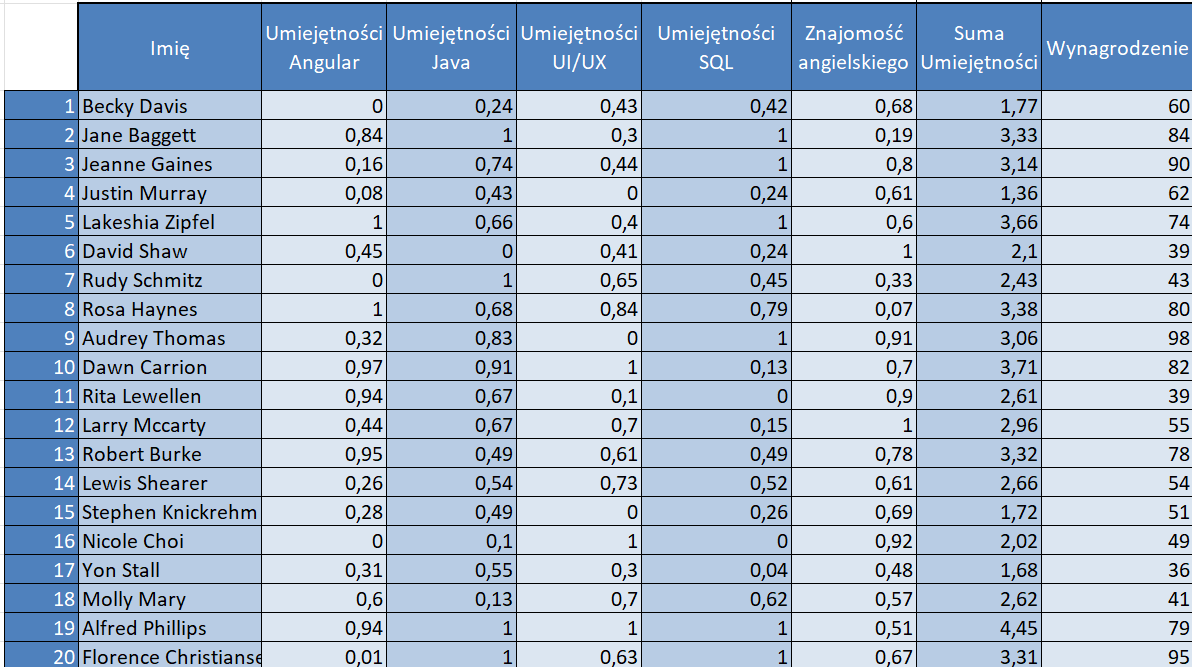
\includegraphics[width=\linewidth]{chapters/Images/pracownicy_csv.png}
    \cprotect\caption{Struktura danych pracowników w pliku \verb|.csv| po wygenerowaniu}
    \textit{Źródło: opracowanie własne}
\end{figure}

\par Tak utworzony zbiór danych stanowi podstawę do analizy możliwości modelu optymalizacyjnego przy różnych warunkach i ograniczeniach w kontekście zarządzania zespołami projektowymi w branży IT. Analiza danych umożliwi wykrycie istotnych wzorców i trendów, które bezpośrednio wpłyną na efektywność i skuteczność optymalnego zespołu projektowego.



\section{Omówienie kodu generatora danych}\label{sec:kod_generator}
\par Kod przedstawiony na grafice pełni rolę generatora danych dla pracowników w kontekście projektu IT. Przede wszystkim, generuje on dane dotyczące umiejętności technicznych i wynagrodzenia pracowników. Poniżej znajduje się szczegółowe omówienie każdej sekcji kodu z uwzględnieniem numeracji linii.

\lstinputlisting[language=Python, caption=Kod źródłowy generatora danych \textit{Źródło: opracowanie własne}]{generator.py}

\begin{description}
    \item[Linie 1-3] - Na początku skryptu importowane są trzy kluczowe biblioteki: \verb|numpy| (alias \verb|np|), \verb|pandas| (alias \verb|pd|) oraz \verb|names|. Biblioteka numpy jest używana do operacji matematycznych i generowania losowych danych, pandas do tworzenia i manipulacji strukturami danych, takimi jak DataFrame, a names do generowania losowych imion pracowników. 
    
    \item[Linie 5-8] Następnie, do linii 8 użytkownikowi wyświetlane są zapytania o wartości kluczowych zmiennych: \verb|liczba_pracownikow, srednia_umiejetnosci, odchylenie_standardowe| oraz \verb|nazwa_pliku_csv|. Od pierwszych trzech zależy finalny wygląd wygenerowanych danych, czwarta określa nazwę pliku do zapisu wyników.
    
    \item[Linie 10-12] W tych liniach tworzony jest słownik \verb |dane_pracownikow|, który początkowo zawiera jedynie losowo wygenerowane imiona pracowników. Imiona są generowane przy użyciu funkcji \verb |names.get_full_name()| w pętli dla wszystkich pracowników.
    
    \item[Linie 14-18] - Następnym krokiem jest zdefiniowanie listy umiejętności (\verb|umiejetnosci|), które będą przypisane do pracowników: \verb|Umiejetnosci Angular, Umiejetnosci Java,| \verb|Umiejetnosci UI/UX, Umiejetnosci SQL| i \verb|Znajomosc angielskiego|. Dla każdej umiejętności w liście, generowane są losowe wartości przy użyciu rozkładu normalnego z określoną średnią i odchyleniem standardowym. Wartości te są zaokrąglane do dwóch miejsc po przecinku i ograniczane do przedziału $[0, 1]$ za pomocą metody \verb|np.clip()|. Po wygenerowaniu danych, lista pracowników jest przekształcona w \verb|DataFrame|.
    
    \item[Linie 19-21] - W tych liniach obliczana jest wartość sumy umiejętności dla każdego pracownika oraz 75. percentyl, na którego podstawie ustalane jest wynagrodzenie. Jeśli suma umiejętności pracownika jest większa od kwantyla sumy umiejętności pracowników, dostaje on wynagrodzenie losowane z przedziału $[70, 99]$. W przypadku wartości niższej wynagrodzenie losowane jest z przedziału $[30, 69]$.
    \item[Linie 23-25] - Na koniec wykonywania skrypt wyświetla pierwsze wiersze pliku z danymi pracowników i wyświetla nazwę pod która plik został zapisany.
\end{description}

\section{Kryteria i ograniczenia modelu}\label{sec:ograniczenia_modelu}
\par Kryteria, które definiują budowę oraz proces tworzenia modelu optymalizacyjnego są ściśle związane z osiągnięciem najwyższej możliwie efektywności zespołu projektowego przy minimalizowaniu kosztów utrzymania takiego zespołu. Te kryteria są odwzorowane pod postaciami funkcji celu, ograniczeń oraz zmiennych decyzyjnych. Funkcja celu dąży do minimalizacji kosztów utrzymania zespołu projektowego przy jednoczesnym zapewnieniu jak największego poziomu umiejętności z każdej kategorii dla zapewnienia jak najwyższej jakości wykonywanego projektu przy określonym budżecie przeznaczonym na pracę.
\par Model przestrzega szeregu ograniczeń, które determinują finalny skład zespołu projektowego. Dla zapewnienia realistycznego scenariuszu zostały przyjęte dwa główne ograniczenia: ograniczenie budżetowe oraz ograniczenie minimalnych umiejętności zespołu. 

\begin{description}
    \item[Ograniczenie minimalnych umiejętności zespołu] - istnieje w celu określenia złożoności projektu. W obecnej branży IT, poziom zaawansowania i stopień trudności wykonania projektu jest wielce zróżnicowany i jego dokładne określenie, może znacząco ułatwić przebieg prac. Odpowiednie dobranie członków zespołu, który ma nad nim pracować, może znacząco ułatwić ten proces. Ograniczenie można przedstawić następującym wzorem:
    \[
        \sum_{i \in \mathcal{P}}^{n} \sum_{Skill \in \mathcal{U}}^{m} i_{Skill} \leq req
    \]
    gdzie:
    \begin{itemize}
        \item $n$ to liczba wszystkich pracowników zawartych w pliku \verb|pracownicy.csv|
        \item $\mathcal{P}$ to zbiór wszystkich pracowników w pliku \verb|pracownicy.csv|
        \item $m$ to liczba umiejętności wyróżnionych w tabeli w pliku \verb|pracownicy.csv|
        \item $\mathcal{U}$ to zbiór wszystkich umiejętności zawartych w tabeli w pliku \verb|pracownicy.csv|
        \item $Skill$ to wartość umiejętności $Skill$ dla pracownika $i$ z zakresu $[0,1]$
        \item $i_{Skill}$ to poziom umiejętności $Skill$ dla pracownika $i$
        \item $req$ to minimalny wymagany poziom umiejętności pracownika w zespole
    \end{itemize}
    
    \item[Ograniczenie budżetowe] - zobowiązuje model do przestrzegania ustalonego budżetu na zespół projektowy. Taki budżet może być określony przez na przykład klienta zlecającego projekt firmie IT lub wewnętrznie przez menadżera zespołu w przypadku gdy zlecenie obejmuje więcej usług niż tylko projekt IT. Budżet jest implementowany poprzez typ integer w celu zapewnienia, że budżet będzie liczbą całkowitą.
    Sprawdzenie czy model spełnia to ograniczenia wiąże się z obliczeniem czy wynagrodzenie godzinowe wybranych pracowników pomnożone przez liczbę godzin na projekt, jest mniejsze od zadanego budżetu. Ograniczenie to można opisać wzorem:
    \[
    \sum_{i \in \mathcal{P}}^{n} (x_i \cdot w_i \cdot h) \leq B
    \]
    
    gdzie:
    \begin{itemize}
        \item $\mathcal{P}$ to zbiór wszystkich pracowników w zbiorze danych
        \item $x_i$ to zmienna decyzyjna określająca, czy pracownik $i$ jest wybrany do zespołu (1 jeśli wybrany, 0 w przeciwnym razie)
        \item $K_i$ to wynagrodzenie godzinowe pracownika $i$
        \item $h$ to liczba godzin pracy nad projektem
        \item $B$ to maksymalny dostępny budżet
        \item $n$ to liczba pracowników w pliku \verb|pracownicy.csv|
    \end{itemize}
\end{description}

\par Oprócz ograniczeń wymaganych do funkcjonalności modelu, istnieją też ograniczenia które nie były dotąd poruszane w jego kontekście i mogą być niejawne, a możliwy jest ich znaczący wpływ na efektywność i skuteczność modelu.

\par Pierwszym z nich jest dostępność i format danych. Wyniki modelu są ściśle związane i zależne od danych wejściowych. Jakość, ilość oraz kompletność danych ma bezpośredni wpływ na końcowy wynik optymalizacji. Jeśli dane są niekompletne, nieprecyzyjne lub zniekształcone model może wygenerować suboptymalne, a w skrajnych przypadkach błędne wyniki. Dlatego też ważnym aspektem przy przeprowadzaniu takiej optymalizacji jest upewnienie się, że dane wejściowe są dokładne i kompletne.

\par Drugim jest mała elastyczność na zmieniające się czynniki i wymagania. Ten model został zaprojektowany dla stałych parametrów i ograniczeń i może nie spełniać swojej funkcji, gdy któraś z tych rzeczy ulegnie zmianie. Na przykład, jeśli budżet lub czas na wykonanie projektu ulegnie zmianie w trakcie trwania projektu, model może wymagać ponownej kalibracji lub nawet całkowitej przebudowy. W praktyce oznacza to, że model powinien być stosowany w przede wszystkim stabilnym środowisku, w którym parametry projektu są dobrze znane i nie są podatne na częste zmiany. W przeciwnym razie, każda zmiana może wymagać modyfikacji modelu, co może prowadzić do zwiększenia kosztów i utraty cennego czasu. 

\par Ostatnim jest preferowanie najniższego kosztu nad jakością zespołu. Priorytetem w obecnej implementacji modelu jest całkowity koszt zespołu ponad jego jakością. Oznacza to, że model będzie tworzył zespoły złożone z mniej wykwalifikowanych pracowników w celu utrzymania jak najniższych kosztów. Mimo tego, że model stara się utrzymać dany poziom umiejętności w zespole, jego głównym celem jest minimalizacja kosztów. W sytuacjach, gdzie jakość jest kluczowym czynnikiem, zastosowanie tego modelu może nie być najlepszym wyborem. W takich sytuacjach, należałoby zaimplementować model w taki sposób, żeby dążył do jak najwyższego poziomu umiejętności w zespole, a sprawa budżetu była drugorzędna.

\par Zrozumienie tych dodatkowych ograniczeń, pozwala na lepsze zrozumienie w jakich sytuacjach i kontekstach model optymalizacyjny najlepiej spełni swoje zadanie. Dodatkowo można dzięki temu zrozumieć i przewidzieć jakie wyzwania może napotkać model w trakcie optymalizacji. Dzięki szerszemu zrozumieniu, można być lepiej przygotowanym do pracy z tym modelem i skuteczniej dobierać dla niego zadania.


\chapter{Studium przypadku}
\par W tym rozdziale poświęconym na studium przypadku, zostanie przeprowadzony eksperyment oparty o wcześniej krótko opisany model optymalizacyjny. Jednocześnie, ten rozdział pokaże pełen proces tworzenia modelu optymalizacyjnego w oparciu o zadany problem oraz jego implementacje w wybranym środowisku. Głównym celem tego eksperymentu jest praktyczne zastosowanie teoretycznych założeń modelu optymalizacyjnego oraz zweryfikowanie jego skuteczności w rzeczywistych warunkach. 
\par Do eksperymentu zostaną wykorzystane dane wygenerowane przez skrypt \verb|generator.py|, który wyprodukuje losowe dane, odzwierciedlające różne scenariusze panujące w firmach IT. Tak wygenerowane dane zostaną użyte jako dane wejściowe dla skryptu \verb|optimizer.py|, który przeprowadzi właściwą optymalizacje składu zespołu projektowego. Optymalizacja będzie mieć na celu uzyskanie takiego zestawu pracowników, który jednocześnie spełnia ograniczenia budżetowe oraz ograniczenia minimalnej sumy umiejętności członków tego zespołu.
\par Dane pozyskane poprzez uruchomienie obu skryptów zostaną poddane analizie statystycznej, której wyniki zostaną dokładnie omówione i przedstawione. Celem analizy będzie zawarcie oceny różnych parametrów takich jak średnia, mediana, odchylenie standardowe, maksimum oraz minimum poszczególnych umiejętności, jak i wynagrodzeń.  Wyniki analiz zostaną dokładnie omówione oraz przedstawione w tabelach oraz na wykresach, co umożliwi bardziej przejrzyste zrozumienie wyników optymalizacji.
\par Na koniec rozdziału zostaną omówione możliwe wady, ograniczenia oraz wyzwania związane z zastosowanym modelem optymalizacyjnym. Przykładowymi mogą być uproszczony model oceny umiejętności pracowników lub brak pełnej reprezentacji rzeczywistych scenariuszy. Zidentyfikowanie tych wad i ograniczeń, może znacząco usprawnić przebieg przyszłych eksperymentów oraz może prowadzić do przyszłych usprawnień modelu.
\par W literaturze istnieje wiele badań na temat zastosowań programowania liniowego oraz badań operacyjnych (ang. Operations Research lub OR) w optymalizacji zarządzania projektami. Przykładem może być praca L. V. Tavares, który pisze "\textit{Badania operacyjne wniosły istotne naukowe wkłady w sukces zarządzania projektami, nie tylko poprzez różnorodne modele pozwalające zrozumieć i przedstawiać projekty, ale także dzięki opracowaniu algorytmów i narzędzi wspierających rolę decyzyjną kierownika projektu.}" \parencite{tavares2002review}. Potwierdza tym znaczenie badań operacyjnych i programowania liniowego w dziedzinie zarządzania projektami,a co za tym idzie zespołami projektowymi. Dzięki temu, zastosowanie OR i LP dla tego eksperymentu jest w pełni uzasadnione i można oczekiwać realnie użytecznych wyników i wniosków.

\section{Zadanie optymalizacyjne jako studium przypadku} \label{sec:studium}
\par W celu zaprezentowania użyteczności wcześniej przedstawionego modelu optymalizacyjnego oraz skryptu służącego do jej przeprowadzania, zostało sporządzone zadanie optymalizacyjne. Zadanie przedstawia problem optymalizacyjny, do którego rozwiązania posłuży wyżej wymieniony model oraz skrypt. Problem zadania polega na minimalizacji kosztów zespołu projektowego w firmie IT, odpowiedzialnego za wykonanie pewnego oprogramowania. Przy minimalizacji kosztów zespołu, muszą być brane pod uwagę ograniczenia w formie budżetu przeznaczonego na projekt oraz jak najwyższej łącznej oceny umiejętności zespołu. Aby zapewnić przejrzyste oraz poprawne wykonanie zadania, problem należy podzielić na części. Oznacza to wcześniejsze wypisanie parametrów i zmiennych decyzyjnych, określenia ograniczeń na ich podstawie oraz wyznaczenia funkcji celu. Te czynności poprzedzają implementacje modelu optymalizacyjnego w środowisku języka Python lub w innym wybranym środowisku (np. środowisko R, MatLab itp.).

    \subsection{Definicja problemu}\label{subsec:problem}
    \par Menedżer projektu ma za zadanie skompletować optymalny zespół pod nowy projekt, którym będzie zajmować się firma. Ma do dyspozycji plik z danymi o pracownikach (\verb|pracownicy.csv|), w którym znajdują się dane o każdym z pracowników. W całej firmie jest 2000 pracowników, którzy mogliby należeć do tego zespołu. Dane przedstawiają poszczególne umiejętności, sumę umiejętności oraz żądane wynagrodzenia na godzinę. Każda z umiejętności jest zapisana jako liczba całkowita z przedziału od 0 do 1, a wynagrodzenia uzależnione jest od wartości sumy umiejętności. Umiejętności podzielone zostały na 5 kategorii: \verb|umiejętności Angular|, \verb|umiejętności Java|, \verb|umiejętności UI/UX|, \verb|umiejętności SQL| oraz \verb|znajomość języka angielskeigo|. Przykładowe wiersze z pliku \verb|pracownicy.csv| wyglądają następująco:
    \begin{figure}[H]
        \centering
        \includegraphics[width=\linewidth]{chapters/Images/pracownicy_przykład.png}
        \cprotect\caption{Przykładowe dane pracowników w pliku \verb|pracownicy.csv|\\ Źródło:\textit{ opracowanie własne}} 
    \end{figure}

    \par Menedżer musi wziąć pod uwagę ograniczenia przy wyborze pracowników, do których należą budżet i minimalny poziom umiejętności zespołu potrzebny do wykonania projektu. Budżet został określony przez dyrektora firmy na 150 000 złotych, a czas na wykonanie projektu stanowi 120 roboczogodzin (dalej RBH). Dla uproszczenie zadania budżet bierze pod uwagę tylko wynagrodzenia pracowników. Z uwagi na złożoność i wymagania jakie stawia wytworzenie tego oprogramowania, menedżer ustalił, że minimalny poziom umiejętności w tym zespole będzie wynosić 85 punktów.
    \par Ręczne przeglądanie 2000 wierszy z danymi i sprawdzanie optymalności zajęłoby zbyt dużo czasu, stąd potrzeba na zastosowanie optymalizacji matematycznej, programowania liniowego i języka programowania Python. Następnymi krokami będzie wypisanie zmiennych i parametrów oraz wyznaczenie funkcji celu i określenie ograniczeń.

    \subsection{Parametry i zmienna decyzyjna}
    \par W tej części zostały wypisane zmienne i parametry, użyte w modelu optymalizacyjnym do wyznaczenia optymalnego składu zespołu projektowego.
    \begin{description}

        \item[Zbiór pracowników] - Zbiór wszystkich pracowników zawartych w pliku \verb|pracownicy.csv|: $\mathcal{P}$

        \item[Liczba pracowników] - Liczba wszystkich pracowników zawartych w pliku \verb|pracownicy.csv|: $n$
    
        \item[Budżet] - Całkowity budżet na wynagrodzenia pracowników: $B = 150 000pln$
        
        \item[Czas na wykonanie projektu] - Całkowita liczba RBH przeznaczona na projekt: $h = 120 RBH$

        \item[Umiejętności pracownika] - Wartość umiejętności $j$ u pracownika $i$ z zakresu $[0, 1]$: $Skill$

        \item[Zbiór umiejętności] - Zbiór wszystkich umiejętności wyróżnionych w tabeli w pliku \verb|pracownicy.csv|: $\mathcal{U}$

        \item[Liczba umiejętności] - Liczba wszystkich umiejętności wyróżnionych w tabeli w pliku \verb|pracownicy.csv|: $5$
        
        \item[Suma umiejętności pracownika] - Wartość sumy wszystkich umiejętności pracownika $i$: 
            \[
                \sum_{Skill \in \mathcal{U}}^{m} i_{Skill} = SumSkill
            \]
        
        \item[Wymagany poziom umiejętności] - minimalny wymagany poziom umiejętności w zespole: $req$
        
        \item[Minimalny poziom umiejętności zespołu] - Minimalna suma umiejętności wszystkich pracowników w zespole jest opisana wzorem:
        
        \[
        \sum_{i \in \mathcal{P}}^{n} SumSkill_{i} = Min_{SumSkill_{i}}
        \]
        
        gdzie \(SumSkill_{i}\) reprezentuje sumę umiejętności \(i\)-tego pracownika.
        
        \item[Koszt godzinowy pracownika] - Kwota wynagrodzenia na godzinę w złotówkach dla \(i\)-tego pracownika: \(K_{i}\)

        \item[Całkowity koszt pracownika] - Całkowita kwota wynagrodzenia za cały przebieg projektu dla \(i\)-tego pracownika: 
            \[
                K_{i} \cdot h
            \]

        \item[Zmienne decyzyjna] - Zmienne binarne określające przydzielenie pracownika do zespołu
            {\begin{itemize}
                \item $x_{i} = 1$ - jeśli pracownik został wybrany do zespołu
                \item $x_{i} = 0$ - jeśli pracownik nie został wybrany do zespołu
            \end{itemize}}
    \end{description}
    
    \subsection{Funkcja celu i ograniczenia}
    \par Po wyznaczeniu zmiennych decyzyjnych i parametrów potrzebnych do stworzenia modelu, należy wypisać ograniczenia oraz sporządzić funkcje celu. 

    \begin{description}
        \item[Ograniczenie budżetowe] Pierwszym z ograniczeń będzie ograniczenie budżetowe. W zadaniu było wyjaśnione, że łączny budżet na wynagrodzenia pracowników nie może przekroczyć 150 000 złotych. Takie ograniczenie, przy przyjętych oznaczeniach, można opisać wzorem:
            \[
                \sum_{i \in \mathcal{P}}^{n} (x_{i} \cdot K_{i} \cdot h) \leq B
            \]
        
        \item[Ograniczenie minimalnego poziomu umiejętności] Następnym ograniczeniem jest minimalny poziom umiejętności zespołu     $Min_{SumSkill_{i}}$, który przy przyjętych oznaczeniach można opisać wzorem:
            \begin{enumerate}
                \item 
                    \[
                        \sum_{i \in \mathcal{P}}^{n} \sum_{Skill \in \mathcal{U}}^{m} i_{Skill} \leq req
                    \]
                \item 
                    \[
                        \sum_{i \in \mathcal{P}}^{n} SumSkill \leq req
                    \]      
                \item 
                    \[
                        Min_{SumSkill_{i}} \leq req
                    \]
                \item 
                    \[
                        Min_{SumSkill_{i}} \leq 85
                    \] 
        \end{enumerate} 
        
        \item[Funkcja celu] Z treści problemu można wywnioskować, że celem optymalizacji zespołu projektowego będzie minimalizacja kosztów całego zespołu, przy jednoczesnym założeniu utrzymania jak najwyższego poziomu umiejętności zespołu. Z  tym wziętym pod uwagę i przy przyjętych oznaczeniach można wyznaczyć funkcje celu takim wzorem:
            \[
               Minimize \sum_{i \in \mathcal{P}}^{n} (x_{i} \cdot K_{i} \cdot h)
            \]
    \end{description}

    \par W tym podrozdziale zostało przedstawione zadanie optymalizacyjne w ramach studium przypadku. Owa optymalizacja została sformułowana jako minimalizacja kosztów zespołu projektowego w firmie IT, która dysponuje danymi o swoich pracownikach w pliku \verb|pracownicy.csv|. Zidentyfikowano kluczowe parametry i zmienne, a także określono funkcje celu oraz jej ograniczenia. Do ograniczeń należało ograniczenie budżetowe oraz ograniczenie minimalnego poziomu umiejętności zespołu, a funkcja celu dąży do minimalizacji kosztu zespołu. Implementacja tego zadania, a co za tym idzie modelu optymalizacyjnego, zostanie przeprowadzona w języku programowania Python z wykorzystaniem bibliotek \verb|PuLP| dla łatwego modelowania oraz \verb|Pandas| dla pracy z plikami csv. 
    
\section{Zastosowanie modelu do optymalizacji zespołu projektowego}
\par W tej części pracy zostanie przeprowadzone badanie problemu opisanego w sekcji \refnote{sec:studium}. Badanie będzie polegało na wygenerowaniu danych o pracownikach za pomocą \verb|generator.py|. Następnie zostanie przeprowadzona analiza wygenerowanych danych za pomocą skryptu \verb|analyzer.py|. Po przeprowadzonej analizie, wygenerowane dane zostaną załadowane do skryptu \verb|optimizer.py|, który dokona optymalizacji problemu, a jej wyniki również zostaną poddane analizę przez skrypt \verb|analyzer.py|. Analizę poprzedzi omówienie kodu analizującego dane, w celu wyjaśnienia działania i metodologii użytej przy analizie wyników.
    
    \subsection{Implementacja modelu optymalizacyjnego}\label{subsec:optimizer_implementacja}
        \par W tej sekcji została szczegółowo omówiona implementacja modelu optymalizacyjnego, który pozwala na efektywne zarządzanie zasobami ludzkimi w firmie IT, z wykorzystaniem technik programowania liniowego. Implementacja ta obejmuje różnorodne narzędzia i technologie, które umożliwiają budowę, rozwiązanie oraz analizę wyników modelu optymalizacyjnego.
    
    \subsubsection{Opis wykorzystanych narzędzi i technologii}
    \par W celu implementacji modelu optymalizacyjnego, zastosowano kilka kluczowych narzędzi i technologii. Każde z tych narzędzi odgrywa istotną rolę w procesie budowy, rozwiązania oraz analizy modelu programowania liniowego. W niniejszej sekcji omówione zostaną najważniejsze z nich.
    \begin{description}
        
        \item[Python] - Python jest językiem programowania wysokiego poziomu, który jest szeroko stosowany w analizie danych, uczeniu maszynowym oraz optymalizacji. Jego prostota i czytelność, w połączeniu z bogatym ekosystemem bibliotek, czynią go idealnym wyborem do realizacji zadań związanych z optymalizacją. Jak podkreśla \parencite{lutz2013learning} w swojej książce, Python jest doskonałym narzędziem dla inżynierów danych ze względu na swoją wszechstronność i dostępność bibliotek wspierających złożone analizy.
        
        \item[Pandas] - Biblioteka pandas jest jednym z najważniejszych narzędzi w ekosystemie Pythona, umożliwiającym łatwe i efektywne przetwarzanie oraz analizę danych. Pandas oferuje struktury danych takie jak DataFrame, które są niezwykle użyteczne w manipulacji dużymi zestawami danych. Twórca Pandas, \parencite{mckinney2013python}, opisuje bibliotekę jako narzędzie, które radykalnie zmienia sposób, w jaki analitycy pracują z danymi, umożliwiając szybkie i intuicyjne operacje na dużych zestawach danych. W niniejszym projekcie pandas jest używane do wczytywania danych pracowników z pliku CSV, ich transformacji oraz przygotowania do dalszej analizy i modelowania.
        
        \item[PuLP] - Jest to biblioteka Python'a do modelowania problemów programowania liniowego. Umożliwia definiowanie zmiennych decyzyjnych, funkcji celu oraz ograniczeń w sposób deklaratywny, a następnie rozwiązywanie tych problemów za pomocą różnych solverów. W tym studium przypadku, PuLP jest wykorzystywane do stworzenia i rozwiązania modelu optymalizacyjnego, który minimalizuje koszty zatrudnienia przy jednoczesnym spełnieniu wymagań dotyczących umiejętności zespołu. Jak wskazuje, Mitchell S. \parencite{mitchell2009introduction}, obszar badań operacyjnych w którym biblioteka PuLP jest przydatna to rozwój i modelowanie problemów LP.
        
        \item[CSV] - Format CSV (Comma-Separated Values) jest powszechnie używany do przechowywania i wymiany danych w formacie tekstowym. W projekcie dane wejściowe pracowników są wczytywane z pliku CSV, a wyniki optymalizacji również zapisywane są w tym formacie, co ułatwia ich późniejszą analizę i interpretację. Format CSV jest prosty i szeroko kompatybilny, co czyni go idealnym wyborem do pracy z danymi w różnych etapach procesu optymalizacji.
        
        \item[Integracja] - Wszystkie te narzędzia i technologie są zintegrowane w celu stworzenia kompletnego systemu optymalizacji. Python, wraz z bibliotekami \verb|pandas| i \verb|PuLP|, umożliwia efektywne przetwarzanie danych, modelowanie problemów programowania liniowego oraz znajdowanie optymalnych rozwiązań. Format CSV zapewnia prosty sposób wymiany danych między różnymi etapami procesu optymalizacji, co ułatwia pracę nad danymi i ich analizę. Dzięki temu możliwe jest stworzenie efektywnego i łatwego w użyciu narzędzia do zarządzania zasobami ludzkimi w firmach IT.
        
    \end{description}
        
    \subsubsection{Omówienie kodu źródłowego modelu optymalizacyjnego}
    \par W tej sekcji rozdziału zostanie szczegółowo omówiony kod źródłowy skryptu optymalizacyjnego, którego celem jest optymalizacja składu zespołu projektowego w firmie IT. Dane pracowników wykorzystane do optymalizacji zostają pobierane z pliku \verb|pracownicy.csv| a następnie zostają wczytane do modelu w celu optymalizacji. Model posiada implementacje ograniczeń opisanych w problemie oraz wyznaczonej funkcji celu, a także zapisuje wyniki optymalizacji w pliku \verb|wybrani_pracownicy.csv| w celu dalszej analizy.

    \lstinputlisting[language=Python, caption={Kod źródłowy modelu. \\Źródło:\textit{ opracowanie własne}}]{optimizer.py}

    \begin{description}
        \item[Linie 1-2] W tych dwóch liniach importowane są biblioteki niezbędne do realizacji modelu optymalizacyjnego, które szczegółowo zostały omówione w poprzednim rozdziale. W środowisku języka \verb|Python|, potrzeba i chęć wykorzystania konkretnej biblioteki wiąże się z jej wcześniejszym zaimportowaniem.
        \item[Linie 4-5] W liniach 4 i 5 skrypt pyta użytkownika o nazwę pliku z danymi pracowników przeznaczonych do optymalizacji (zmienna \verb|sciezka_do_pliku|) oraz o nazwę pliku, który służy do przechowania wyników optymalizacji (zmienna \verb|nazwa_pliku_csv|).
        \item[Linie 9-11] W tych liniach użytkownik jest proszony o podanie wartości dla zmiennych \verb|budzet, liczba_godzin_projektu| oraz \verb|minimalne_umiejetnosci|. Te trzy linie są kluczowe dla powodzenia optymalizacji, gdyż na ich podstawie są ustalane ograniczenia.
        \item[Linie 13-14] Następnie jest tworzony nowy problem optymalizacyjny nazwany \verb|Optymalizacja_zespolu_projektowego|, który będzie dążyć do minimalizacji łącznego kosztu zespołu. Po utworzeniu modelu, jest zdefiniowana zmienna binarna \verb|x_{i}| służąca do określenia, czy pracownik został wybrany do zespołu (wartość 1), czy też nie został wybrany do zespołu (wartość 0).
        \item[Linie 16-19] W linii 16 definiowana jest funkcja celu opisana wcześniej, definiująca całkowity koszt jako sumę wynagrodzeń pracowników. Następnie dodawane są ograniczenia budżetowe oraz minimalnego poziomu umiejętności opisane we wcześniejszych sekcjach. Ograniczenie budżetowe oblicza łączny koszt wynagrodzeń i zapewnia, że jest mniejsze lub równe założonemu budżetowi. Minimalna suma umiejętności natomiast, czy suma umiejętności wybranych pracowników jest większa lub równa założonemu poziomowi. Następnie model jest rozwiązywany za pomocą metody \verb|solve()|.
        \item[Linie 21-24] W tych liniach, po zakończonej optymalizacji, pobierane są informacje na temat statusu modelu (\verb|status|), o indeksach wybranych pracowników (\verb|wybrani_pracownicy_indeksy|) oraz łącznego kosztu po optymalizacji (\verb|laczny_koszt|).
        \item[Linie 26-36] Te linie zwracają informacje w formie tekstowej na temat statusu modelu, listę wybranych pracowników i ich ilości, imiona wybranych pracowników oraz informacje o łącznym koszcie. Na koniec, skrypt zapisuje uzyskane wyniki do pliku .csv o podanej wcześniej przez użytkownika nazwie. Struktura danych w pliku zawierającym wyniki prezentuje się w następujący sposób: 
            \begin{figure}[H]
                \centering
                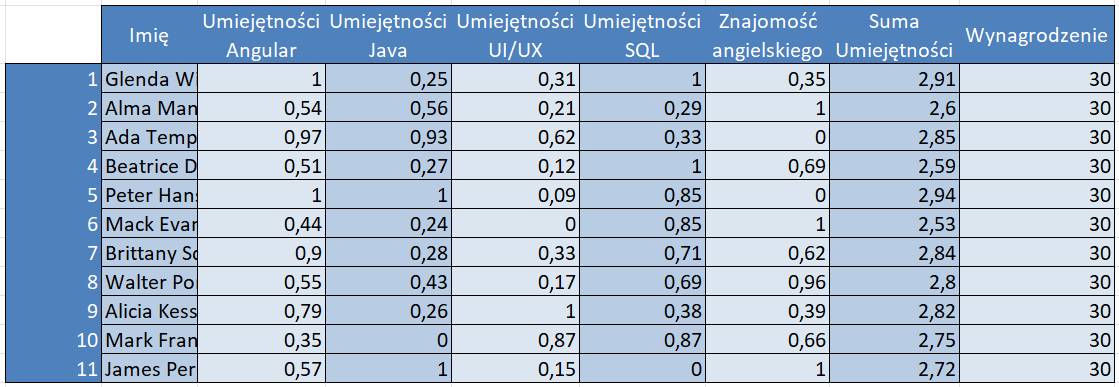
\includegraphics[width=\linewidth]{chapters/Images/wybrani_pracownicy_przyklad_csv.png}
                \cprotect\caption{Przykładowe dane w pliku \verb|wybrani_praocwnicy.csv|\\ Źródło:\textit{ opracowanie własne}}
            \end{figure}
    \end{description}
    
    \par W ten sposób kod realizuje zadanie optymalizacji składu zespołu projektowego, minimalizując koszty przy jednoczesnym spełnieniu wymagań dotyczących umiejętności i budżetu. W następnych sekcjach tego rozdziału zostanie przeprowadzona dokładna analiza statystyczna danych wszystkich pracowników jak i wyników po przeprowadzonej optymalizacji, która posłuży do wyciągnięcia wniosków. Dzięki analizie będzie można określić wady oraz zalety modelu, a także jego użyteczność w bardziej rzeczywistych scenariuszach.

    \subsection{Generacja danych o pracownikach}\label{sec:generacja_danych}
    \par Generowanie danych o pracownikach jest istotnym etapem w testowaniu modelu optymalizacyjnego i przeprowadzania symulacji. Skrypt \verb|generator.py|, opisany w sekcji \refnote{sec:kod_generator}, pozwala na szybkie i efektywne tworzenie losowych danych, które będą używane w dalszych analizach. Korzystanie z losowo generowanych danych umożliwia elastyczne testowanie różnych scenariuszy i pozwala sprawdzić wszechstronność modelu.
    
    \par Przed wygenerowaniem danych, należy upewnić się, że system posiada odpowiednie wymagania programowe. Do takowych należą:
    \begin{description}
        \item[System operacyjny] Windows, macOS lub Linux
        \item[Python] Wersja języka Python 3.11 lub nowsza 
    \end{description}
    Dodatkowo, należy zainstalować biblioteki wymagane do działania skryptu:
    \begin{itemize}
        \item Pandas
        \item NumPy
        \item Names
    \end{itemize}
    
    \lstinputlisting[language=bash, firstline=5, lastline=5, caption=Komenda instalacji bibliotek dla skryptu generatora danych \\Źródło:\textit{ opracowanie własne}]{snippets.sh}
    
    \par Aby wygenerować dane, koniecznym jest podanie kilku znaczących parametrów, takich jak liczba pracowników oraz średnia i odchylenie standardowe, które zostaną użyte w rozkładzie normalnym. W tym badaniu przyjęto następujące wartości:
    
    \begin{itemize}
        \item \verb|liczba_pracowników = 2000|
        \item \verb|srednia_umiejetnosci = 0.4|
        \item \verb|odchylenie_standardowe = 0.5|
    \end{itemize}
    
    Implementacja w skrypcie wygląda następująco, użytkownik zostanie zapytany o wartości tych zmiennych oraz nazwę pliku do zapisania danych:
    
    \lstinputlisting[language=Python, firstline=5, lastline=8, caption=Implementacja zmiennych generatora danych\\ Źródło:\textit{ opracowanie własne}]{generator.py}
    
    \par Rozkład normalny został wybrany ze względu na swoje właściwości statystyczne, które zapewniają, że większość wygenerowanych wartości będzie skupiona wokół średniej. Tak przygotowany skrypt jest gotowy do generowania danych i należy go uruchomić poprzez komendę w terminalu lub za pomocą odpowiedniego przycisku w wybranym środowisku programistycznym. Na potrzeby badania plik z danymi został nazwany \verb|pracownicy.csv|. Wygenerowane dane zostaną zapisane we wcześniej nazwanym pliku w folderze, w którym znajduje się skrypt.
    
    \lstinputlisting[language=bash, firstline=1, lastline=1, caption=Komenda do uruchomienia skryptu generatora\\ Źródło:\textit{ opracowanie własne}]{snippets.sh}


\begin{lstlisting}[language=bash, caption=Terminal po zakończeniu skryptu\\ Źródło:\textit{ opracowanie własne}]
        Imie  Umiejetnosci Angular  Umiejetnosci Java
0   Christina Roll            0.20               0.46
1   Robert Schmitt            0.42               0.00
2       Joshua Key            0.97               0.85
3  Louise Hilliard            0.33               0.71
4  Shelby Mainolfi            1.00               0.09
Dane zostaly zapisane w pliku pracownicy.csv
\end{lstlisting}
    
    \par Dzięki łatwej modyfikacji skryptu, wielokrotne testowanie przy różnych scenariuszach optymalizacyjnych jest wyjątkowo proste i szybkie. Możliwość dokonywania szybkich zmian w procesie generowania danych daje dużą swobodę i pozwala na sprawdzenie modelu przy różnych parametrach wejściowych. 
    
        

    \subsection{Uruchomienie modelu optymalizacyjnego}
    \par Aby poprawnie przystąpić do optymalizacji trzeba wcześniej upewnić się, że system na którym będzie uruchomiony skrypt \verb|optimizer.py| spełnia odpowiednie wymagania. Należą do nich:
        \begin{description}
            \item[System operacyjny] Windows, macOS lub Linux
            \item[Python] Wersja języka Python 3.11 lub nowsza 
        \end{description}
        Dodatkowo, będą potrzebne dwie biblioteki, aby skrypt działał poprawnie:
        \begin{itemize}
            \item Pandas
            \item PuLP
        \end{itemize}
    Można je zainstalować używając komendy:
    \lstinputlisting[language=bash, firstline=7, lastline=7, caption=Instalacja bibliotek potrzebnych dla skryptu optymalizacyjnego\\ Źródło:\textit{ opracowanie własne}]{snippets.sh}

    \par Implementacja oraz optymalizacja modelu za pomocą skryptu \verb|optimizer.py| jest kluczowa w kontekście studium przypadku i przedstawionego problemu. Skrypt umożliwia optymalizacje zasobów pod kątem łącznego kosztu zespołu i jednocześnie zachowuje ograniczenia budżetowe oraz minimalnych umiejętności zespołu. Poprzez pobieranie danych o budżecie, godzinach przeznaczonych na projekt oraz minimalnej sumy umiejętności bezpośrednio od użytkownika, model można uruchomić szybko i sprawnie. W celu uruchomienia skryptu należy w terminalu wpisać komendę:
    
    \lstinputlisting[language=bash, firstline=3, lastline=3, caption=Komenda do uruchomienia skryptu optymalizacyjnego\\ Źródło:\textit{ opracowanie własne}]{snippets.sh}

    \par Po uruchomieniu użytkownik zostaje poproszony o podanie ścieżki do pliku z danymi pracowników oraz o nazwę pliku w którym mają być zapisane wyniki. Na potrzeby badania plik wejściowy nazwano \verb|pracownicy.csv|, a wyniki są zapisywane w pliku \verb|wybrani_pracownicy.csv|. Następnie zostają wprowadzone wartości zmiennych budżet, liczba godzin na projekt oraz minimalna suma umiejętności w zespole. Po podaniu tych parametrów, optymalizacja będzie wykonana, a wyniki zostaną zapisane pod podaną wcześniej nazwą, w tym samym folderze w którym umieszczony jest skrypt.

    \par Po zakończeniu, skrypt wypisuje do konsoli następujące informacje:

\begin{lstlisting}[language=bash, caption=Terminal po zakończeniu skryptu\\ Źródło:\textit{ opracowanie własne}]
Status: Optimal
Wybrani pracownicy:
                     Imie
43        Michael Mccloud
63          Janine Sheats
97           Ronald Brown
124         Edward Roblez
152         Felice Hussey
216           Kent Mendez
350        Carrie Waggner
368        Charles Parker
458           Susan Tracy
488         Teresa Berube
585   Jacqueline Schulman
636             Glenda Le
815           Naomi Hasse
921       Genevieve Posey
926          John Luevano
1024          Floyd Adams
1038           Dana Helms
1067           Emma Wheat
1144           Wanda Hunt
1221           John Truax
1338          Gale Wesley
1371      Breanna Mcguire
1459       Brandy Schmidt
1462        James Pullins
1509        Thomas Walker
1574          Andrea Lien
1625         Emily Walton
1655         James Morgan
1698          Mary Butera
1784           Jay Lerman
1832       Laura Colosimo
1875        Charles Miles
1989          Darrin Berg

Liczba wybranych pracownikow: 33

Laczny koszt: 126000.0
Suma umiejetnosci wybranych pracownikow: 85.02
\end{lstlisting}
    
    Można na nich zauważyć kluczowe informację:
    \begin{description}
        \item[Status: Optimal] - Zwrócona informacja o statusie optymalizacji, \verb|Optimal| oznacza pomyślne wykonanie optymalizacji i informuje o znalezieniu optymalnego rozwiązania problemu.
        \item[Liczba wybranych pracowników] - Informacja o liczbie wybranych pracowników, poprzedzona listą wszystkich pracowników należących do optymalnego zespołu.
        \item[Łączny koszt] - Kolejna znacząca informacja w kontekście badania. Ta wiadomość pokazuje, jaki jest całkowity koszt wynagrodzeń optymalnego zespołu. Maksymalnym budżetem było $150 000$, więc można zauważyć, że skrypt już zaoszczędził $24 000$ złotych.
        \item[Suma umiejętności] - Ta linia informuje o sumie umiejętności w zespole, w którym wymagane było przynajmniej 85 punktów umiejętności.
    \end{description}
    

\section{Analiza wyników i wnioski}\label{sec:analiza}
\par Przeprowadzenie analizy danych populacji pracowników oraz pracowników wybranych przez model optymalizacyjny jest kluczowe dla rozwiązania problemu opisanego w rozdziale \ref{sec:studium} na stronie \pageref{sec:studium} oraz dla stwierdzenia użyteczności modelu. Do przeprowadzenia analizy wykorzystano skrypt \verb|analyzer.py|. Posłużono się skryptem w celu uzyskania wyników szybciej, niż w przypadku "ręcznej" analizy danych i manualnego tworzenia wykresów. Czyni to proces oceny pracowników oraz optymalizacji zespołu bardziej wydajnym i przez to optymalnym.

\par Skrypt \verb|analyzer.py| został zaprojektowany po to, żeby automatycznie przetwarzać dane generowane przez \verb|generator.py| oraz wyniki z \verb|optimizer.py|. Przyspiesza on analizę wyników obu skryptów oraz zmniejsza ryzyko błędów spowodowanych przez manualną analizę tych danych. Dodatkowo, skrypt analizujący został stworzony tak, żeby współgrać z modelem optymalizacyjnym oraz generatorem danych, co pozwala na łatwe i szybkie aktualizowanie wytycznych dla skryptu w przyszłości w przypadku zmian w jednym z pozostałych skryptów. 

\par W efekcie, \verb|analyzer.py| jest kluczowym narzędziem w procesie analizy wyników optymalizacji i danych wejściowych oraz jest fundamentem dla przyszłych badań na podobnym lub udoskonalonym modelu. Łatwość obsługi i modyfikacji skryptu pozwala użytkownikom sprawnie dostosowywać skrypt do zmieniających się potrzeb i wytycznych w firmach z sektora IT.

    \subsection{Omówienie kodu źródłowego analizatora}\label{sec:analyzer}
        \par Analiza danych wygenerowanych poprzez \verb|generator.py| została przeprowadzona za pomocą skryptu \verb|analyzer.py|. Skrypt ten przyjmuje plik w formacie \verb|.csv| i konwertuje je do formatu \verb|xlsx|, czyli popularnego arkusza kalkulacyjnego Microsoft Excel. Dostęp do pliku jest uzyskiwany poprzez bibliotekę \verb|Pandas|, a do wizualizacji i analizy statystycznej używane są biblioteki \verb|matplotlib.pyplot| oraz \verb|seaborn|. Funkcjonalność dodawania wykresów jest uzyskana dzięki bibliotekom \verb|xlsxwriter| oraz modułowi języka Python \verb|IO|, a konwersja z .csv na .xlsx jest wykonana dzięki kolejnemu modułowi - \verb|OS|. Kod źródłowy dla \verb|analyzer.py| wygląda w następujący sposób:

        \lstinputlisting[language=Python, caption=Kod źródłowy skryptu analizującego\\ Źródło:\textit{ opracowanie własne}]{analyzer.py}

        \begin{description}
            \item[Linie 1-6] Importowanie potrzebnych bibliotek.
            \item[Linie 8-20] Przygotowanie danych. Skrypt pyta o nazwę pliku do analizy oraz nazwę jaka ma być nadana dla pliku z wynikami. Następnie dane z pliku .csv są konwertowane na format .xlsx i wczytywane do \verb|DataFrame| za pomocą biblioteki \verb|Pandas|.
            \item[Linie 22-24] W tym momencie dane są przygotowywane do analizy. Ustawiane są nazwy kolumn oraz usunięta zostaje całkowicie kolumna o nazwie \verb|Imie|, gdyż nie jest potrzebna do analizy. 
            \item[Linie 27-29] Wymagane jest pogrupowanie wszystkich kolumn na kolumny zawierające dane z poszczególnych umiejętności (\verb|skills_columns|) oraz na wszystkie kolumny (\verb|numeric_columns|). Po podziale, dane są konwertowane do typu numerycznego.
            \item[Linie 30-34] W tych liniach obliczane są podstawowe statystyki zbioru danych poprzez metodę \verb|desscribe()| dla każdej kolumny z grupy \verb|numeric_columns|. Osobno są też obliczane mediana (\verb|means|) i odchylenie standardowe (\verb|std_devs|).
            \item[Linie 36-44] Te linie odpowiadają za utworzenie nowego pliku Excel o wcześniej podanej przez użytkownika nazwie oraz zapisanie do niego statystyk obliczonych w liniach \verb|20 - 24| do arkusza o nazwie \verb|Statistics|. Następnie skrypt tworzy obiekt\verb|workbook| i dodaje do niego arkusz \verb|Plots|, który jest przypisany do obiektu \verb|worksheet| używanego do zapisywania wykresów. Odniesienia do wszystkich arkuszy z pliku Excel przechowywane są w słowniku \verb|writer.sheets|, a dodanie \verb|worksheet| do tego słownika pozwala na późniejsze odniesienie się do tego arkusza poprzez nazwę \verb|Plots|. Zmienne \verb|row| oraz \verb|col| to zmienne ideksujące pozycję arkuszy w Excelu. Będą wykorzystywane do ustalenia pozycji umieszczanych wykresów.
            \item[Linie 46-59] W tej pętli tworzone są histogramy z krzywą gęstości dla każdej kolumny \verb|numeric_columns| oraz zapisanie tych obrazów do arkusza Excel w indeksach wyznaczonych przez zmienne \verb|col| i \verb|row|.
            \item[Linie 61-72] W tym fragmencie tworzona jest macierz korelacji pomiędzy wartościami z kolumn w grupie \verb|numeric_columns|.
            \item[Linie 74-86] Tutaj tworzony jest wykres rozrzutu wynagrodzenia w zależności od sumy umiejętności.
            \item[Linia 88] Na koniec wyświetlany jest komunikat o zakończeniu analizy.
        \end{description}

        \par Do uruchomienia skryptu analizującego, wymagane jest, aby system użytkownika spełniał kilka wymagań, którymi są:

        \begin{description}
            \item[System operacyjny] Windows, macOS lub Linux
            \item[Python] Wersja języka Python 3.11 lub nowsza 
        \end{description}
        Dodatkowo, będą potrzebne różne biblioteki, aby skrypt działał poprawnie:
        \begin{itemize}
            \item Pandas
            \item matplotlib.pyplot
            \item seaborn
            \item xlsxwriter
        \end{itemize}
        Można je zainstalować używając tej komendy w terminalu:
        
        \lstinputlisting[language=bash, firstline=9, lastline=9, caption=Instalacja bibliotek dla skryptu analizującego\\ Źródło:\textit{ opracowanie własne}]{snippets.sh}

        \par Po przeprowadzonej instalacji, należy uruchomić skrypt poprzez naciśnięcie odpowiedniego przycisku w wybranym środowisku programistycznym lub poprzez wpisanie tej komendy w terminalu:

        \lstinputlisting[language=bash, firstline=2, lastline=2, caption=Komenda do uruchomienia skryptu analizującego\\ Źródło:\textit{ opracowanie własne}]{snippets.sh}

        \par Uruchomienie skryptu spowoduje pojawienie się pytań do użytkownika o:
        \begin{itemize}
            \item Nazwę pliku do analizy
            \item Nazwę pliku, w którym mają zostać zapisane wyniki. na potrzeby badania została nadana nazwa \verb|analiza_pracownicy|.
        \end{itemize}
        Po zakończonej analizie, plik z wynikami zostanie zapisany w folderze, w którym znajduje się skrypt. Tak przeprowadzona analiza zajmuje bardzo mało czasu i dostarcza bezbłędne wyniki do dalszej interpretacji.

\begin{lstlisting}[language=bash, caption=Terminal po zakończeniu skryptu\\ Źródło:\textit{ opracowanie własne}]
Przekonwertowano pracownicy.csv na pracownicy.xlsx
Analiza zakonczona i zapisana w analiza_pracownicy.xlsx    
\end{lstlisting}

    \subsection{Interpretacja analizy wygenerowanych danych pracowników}\label{subsec:analiza_wejscie}
    \par Dane na temat populacji pracowników przeanalizowane przez skrypt \verb|analyzer.py| znajdują się w pliku \verb|.xlsx| o nazwie podanej przez użytkownika. Analiza została podzielona na dwa arkusze: pierwszy - \verb|Statystyki| zawiera podstawową analizę statystyczną danych pracowników w formie tabeli, drugi - \verb|Wykresy| zawiera wygenerowane histogramy, macierz korelacji oraz wykres rozrzutu.

    \subsection{Analiza danych z tabeli}\label{subsec:tabela_populacja}
    \par Tabela przedstawiona na rysunku \ref{fig:tabela_analiza} przedstawia zestawienie statystyk obliczonych przez skrypt \verb|analyzer.py| omówiony w sekcji \refnote{sec:analyzer}. Zawiera ona metryki dla poszczególnych umiejętności oraz wynagrodzenia pracowników. Wśród nich znajdują się:
    \begin{description}
        \item[count] - Liczba pracowników w populacji
        \item[mean] - Średnia
        \item[std] - Odchylenie standardowe
        \item[min] - Wartość minimum
        \item[25\%, 50\%, 75\%] - Kwartyl I, kwartyl II oraz kwartyl III
        \item[max] - Wartość maksimum
    \end{description}

    \begin{figure}[H]
        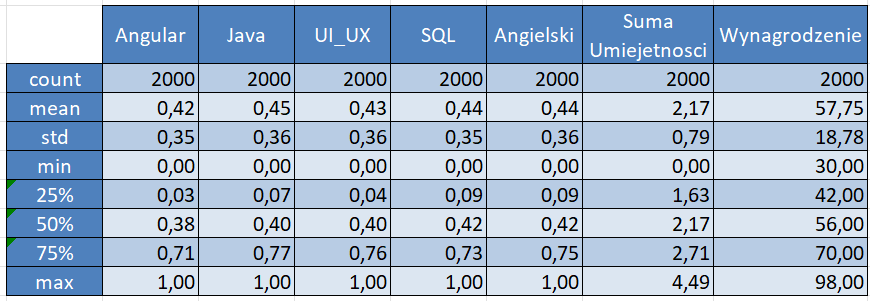
\includegraphics[width=\linewidth]{chapters/Images/analiza_tabela_all.png}
        \cprotect\caption{Tabela populacji pracowników po analizie\\ Źródło:\textit{ opracowanie własne}}
        \label{fig:tabela_analiza}
    \end{figure}

    \par Z tak wygenerowanej tabeli można wyciągnąć następujące wnioski:
    \begin{description}
        \item[Rozmiar populacji\label{itm:count}]  - Pokazuje rozmiar populacji i potwierdza, że analiza została przeprowadzona na pełnym zestawie danych.
        
        \item[Średnia\label{itm:mean}] - Średnia z każdej umiejętności wynosi od $0,42$ do $0,45$, co sugeruje, że większość pracowników posiada średni poziom umiejętności w każdej kategorii. W porównaniu do maksimum poszczególnych umiejętności, znaczna część pracowników posiada niższy o ponad połowę skali poziom umiejętności, niż maksymalny w populacji. Takie średnie są powodem dla średniej sumy pięciu umiejętności równej $2,17$. Natomiast średnia wynagrodzenia jest równa $57,75$ na godzinę, co daje dobre pojęcie o tym, jakiego wynagrodzenia średnio oczekują pracownicy tej firmy i może sugerować, że pracownicy z wyższą sumą umiejętności będą oczekiwać wyższego wynagrodzenia.
        
        \item[Odchylenie standardowe\label{itm:std}] - Odchylenie std. każdej umiejętności będące na dosyć wysokim poziomie $[0,35; 0,36]$, wskazuje na duże zróżnicowanie w poziomach opanowania poszczególnych umiejętności przez pracowników. Co za tym idzie, odchylenie std. dla sumy umiejętności wynoszące $0,79$ jest wysokie  i wskazuje na dużą zmienność w łącznym poziomie umiejętności wśród populacji pracowników firmy. Podobnie w wypadku wynagrodzenia, gdzie odchylenie std. wynosi $18,78$ będąc również na wysokim poziomie. W porównaniu do maksimum żądanego wynagrodzenia wynoszącego $98,00$, takie odchylenie sugeruje obecność dużego zróżnicowania w kwestii wynagrodzenia w populacji i może być spowodowane różnicami w umiejętnościach i sumie umiejętności.
        
        \item[Minimum\label{itm:min}] - Minimalne wartości w poszczególnych kategoriach wynoszą $0$, co dowodzi, że niektórzy pracownicy nie posiadają żadnych umiejętności w danej kategorii. Minimalne wynagrodzenie wynosi $30,00$ co nasuwa wnioski, że najmniej zarabiają pracownicy, o najmniejszej sumie umiejętności.
        
        \item[Maksimum\label{itm:max}] - Maksymalne wartości w poszczególnych kategoriach umiejętności wynoszą $1,00$, co sugeruje istnienie pracowników, którzy opanowali pewne dziedziny w pełni. Jednak można zauważyć, że w populacji nie ma pracownika, który by opanował każdą z umiejętności, gdyż maksymalna suma umiejętności wynosi $4,49$. Natomiast maksymalne wynagrodzenie wynoszące $98,00$, świadczy o obecności pracowników, którzy bardzo cenią swoja wysoką ekspertyzę. Wysoki poziom umiejętności jest ważny, jednak wysokie koszty takich pracowników, mogą ich wyeliminować z końcowego zespołu.
        
        \item[Kwartyle 25\%, 50\% i 75\%\label{itm:kwartyl}] - Kwartyle pokazują jaki rozkład mają poszczególne statystyki i pokazują rozproszenie wartości są rozproszone w populacji pracowników. 
            \begin{itemize}
                \item W kwartylu pierwszym (25\%) umiejętności są na poziomie od $0,3$ do $0,9$, co oznacza istnienie znacznej grupy pracowników o bardzo niskich umiejętnościach i ich sumie, która jest równa lub niższa $1,63$. W kwestii wynagrodzenia, w kwartylu pierwszym pracownicy nie żądają więcej niż $42,00$, co czyniłoby ich dobrymi kandydatami do zespołu, gdyby nie niska suma umiejętności.
                \item W kwartylu drugim (50\%) umiejętności mają wartości pomiędzy $0,38$ a $0,42$, co sugeruje istnienie sporej grupy pracowników o umiejętnościach zbliżonych do średniej i o sumie umiejętności wynoszącej $2,17$, która jest równa średniej sumie umiejętności. W kwestii wynagrodzenia, pracownicy z kwartylu drugiego oczekują wynagrodzenia na poziomie bardzo zbliżonym do średniej równego $56,00$. Takie dane mogą sugerować, że w kwartylu drugim znajdują się pracownicy dobrze pasujący do zespołu omawianego w problemie.
                \item Kwartyl trzeci obejmuje pracowników z umiejętnościami na poziomie poniżej około od $0,71$ do $0,76$. Wiadomo dzięki temu, że tylko 25\% pracowników ma umiejętności na wyższym poziomie niż ta grupa. Suma umiejętności w tym kwartylu wynosi $2,71$ i jest znacznie (o $0,54$) większa od średniej sumy. Wynagrodzenie natomiast wynosi $70,00$, co jest logicznym wynikiem, że większe umiejętności wiążą się z większym oczekiwanym wynagrodzeniem.
            \end{itemize}
        
    \end{description}
    \par Dzięki takie analizie, można wyciągnąć silne wnioski na temat tego, kto zostanie wybrany do zespołu i jak będą wyglądać statystyki takiego zespołu. Optymalnie wybrani pracownicy będą oczekiwali wynagrodzenia z kwartyla drugiego, co wiąże się z niższą ekspertyzą w niektórych kategoriach.
    
    \subsection{Histogramy}\label{subsec:histogramy}
    \par Histogramy przedstawiają częstotliwość występowania pracowników o danych poziomach umiejętności, wynagrodzenia czy sumy umiejętności. Oś X, przedstawia zakres poziomu umiejętności wynosi $[0, 1]$, a oś Y reprezentuje częstotliwość występowania pracowników z określonym poziomem dla danej kategorii w konkretnym zakresie. W przypadku histogramów sumy umiejętności oraz wynagrodzenia oś X przedstawia kolejno zakresy $[0, 5]$ oraz $[0, 100]$. Osie Y w tych wypadkach pozostają niezmienne. Badanie histogramów może wpłynąć na polityki wynagrodzeń oraz na strategie rozwoju firmy. Histogramy pozwolą wyłonić jakie obszary wymagają poprawy oraz pomogą w lepszym docenianiu pracowników z wyższymi umiejętnościami, promując rozwój.
    
        \subsubsection{Umiejętności w kategorii Angular}
        \begin{figure}[H]
            \centering
            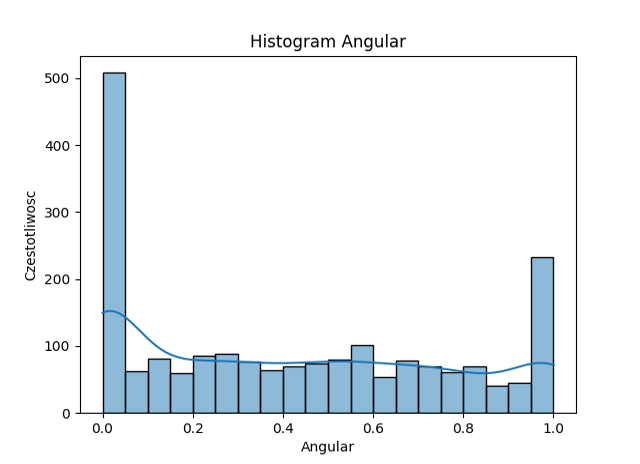
\includegraphics[width=\linewidth]{chapters/Images/hist_angular.png}
            \cprotect\caption{Histogram umiejętności w kategorii Angular\\ Źródło:\textit{ opracowanie własne}}
            \label{fig:hist_angular}
        \end{figure}

        \begin{enumerate}
            \item Występowanie najwyższych słupków przy wartościach $0$ i $1$ oznacza, że wielu pracowników (około 500 dla wartości $0$ i około 250 dla wartości $1$) posiada minimalnym lub maksymalny poziom umiejętności. Stanowi to, że około $25\%$ pracowników nie posiada umiejętności w tej kategorii, a około $12,5\%$ posiada bardzo wysoki poziom zaawansowania.
            \item Rozkład poziomu umiejętności $[0,1; 0,9]$ jest stosunkowo równomierny, z minimalną fluktuacją. Pokazuje to, że w tym przedziale umiejętności znajduje się największa część populacji (około $1250$) i jednocześnie, że mały odsetek populacji posiada średnie umiejętności w tej kategorii. Wartości zbliżone do średniej posiada około $150$ pracowników.
            \item Krzywa gęstości potwierdza obserwacje z poprzedniego punktu, mówiące o rozkładzie umiejętności w populacji, głównie w przedziale $[0,1; 0,9]$ z około $37,5\%$ populacji rozłożonej przy wartościach $0$ i $1$.
        \end{enumerate}
        
        \subsubsection{Umiejętności w kategorii Java}
        \begin{figure}[H]
            \centering
            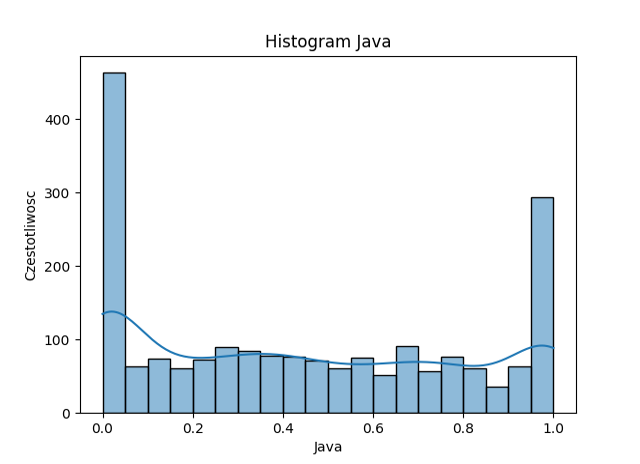
\includegraphics[width=\linewidth]{chapters/Images/hist_java.png}
            \cprotect\caption{Histogram umiejętności w kategorii Java\\ Źródło:\textit{ opracowanie własne}}
            \label{fig:hist_java}
        \end{figure}

        \begin{enumerate}
            \item Podobnie jak przy kategorii Angular najwyższe słupki występują przy wartościach $0$ i $1$ co oznacza, że wielu pracowników (około $450$ dla wartości $0$ i około $300$ dla wartości $1$) posiada tę umiejętność na poziomie równym $0$ lub $1$. Stanowi to, że około $22,5\%$ pracowników nie posiada umiejętności w tej kategorii, a około $15\%$ posiada bardzo wysoki poziom zaawansowania.
            \item Rozkład poziomu umiejętności $[0,1; 0,9]$ jest stosunkowo równomierny, z minimalną fluktuacją. Wskazuje to, że znaczna część populacji (około $1250$) posiada umiejętności w tym zakresie, a umiejętności zbliżone do średniej posiada około $170$ pracowników.
            \item Obserwacja krzywej gęstości daje takie same wnioski, mówiące o rozkładzie umiejętności w populacji, jako zdominowanej przez wartości z przedziału $[0,1; 0,9]$, a resztą skupioną przy wartościach $0$ i $1$.
        \end{enumerate}
        
        \subsubsection{Umiejętności w kategorii UI/UX}
        \begin{figure}[H]
            \centering
            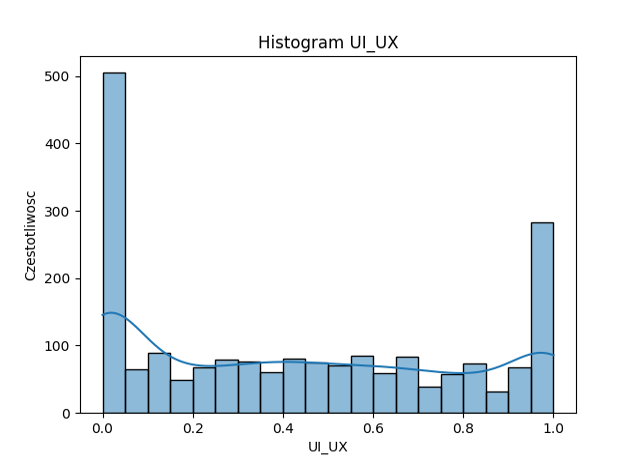
\includegraphics[width=\linewidth]{chapters/Images/hist_uiux.png}
            \cprotect\caption{Histogram umiejętności w kategorii UI/UX\\ Źródło:\textit{ opracowanie własne}}
            \label{fig:hist_uiux}
        \end{figure}

        \begin{enumerate}
            \item Bardzo zbliżone wnioski można wyczytać z histogramu kategorii UI/UX. Najwyższe słupki występują przy wartościach $0$ i $1$ co oznacza, że wielu pracowników (około $500$ dla wartości $0$ i około $300$ dla wartości $1$) posiada tę umiejętność na poziomie równym $0$ lub $1$. Dowodzi to, że około $25\%$ pracowników nie posiada umiejętności w tej kategorii, a około $15\%$ posiada bardzo wysoki poziom zaawansowania.
            \item Rozkład poziomu umiejętności $[0,1; 0,9]$ jest dosyć równomierny. Minimalna fluktuacja wskazuje, że znaczna część populacji (około $1200$) posiada umiejętności w tym zakresie, a umiejętności zbliżone do średniej posiada około $180$ pracowników. Obserwacja krzywej gęstości potwierdza te wnioski i nie wnosi nowych.
        \end{enumerate}
        
        \subsubsection{Umiejętności w kategorii SQL}
        \begin{figure}[H]
            \centering
            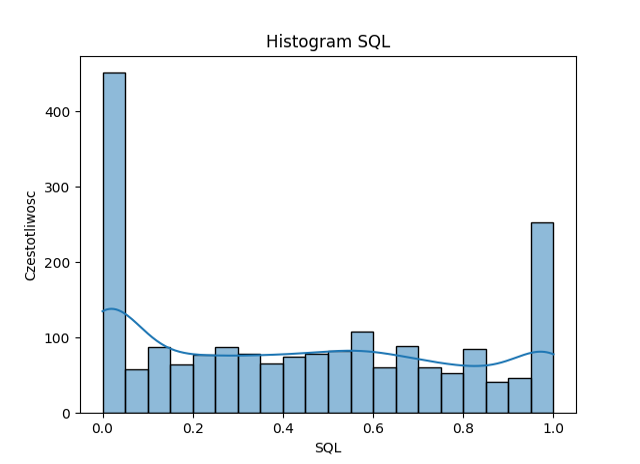
\includegraphics[width=\linewidth]{chapters/Images/hist_sql.png}
            \cprotect\caption{Histogram umiejętności w kategorii SQL\\ Źródło:\textit{ opracowanie własne}}
            \label{fig:hist_sql}
        \end{figure}

        \begin{enumerate}
            \item Histogram kategorii SQL wskazuje na podobny wzorzec jak w poprzednich przypadkach. Wysokie słupki dla wartości $0$ (około $450$ pracowników) i $1$ (około $250$ pracowników), ze znaczną częścią populacji (około $1700$ lub $65\%$ pracowników) z umiejętnościami w przedziale $[0,1; 0,9;]$. Blisko średniej znajduje się około $180$ pracowników. Krzywa gęstości potwierdza te obserwacje.
        \end{enumerate}
        
        \subsubsection{Umiejętności w kategorii Znajomość języka angielskiego}
        \begin{figure}[H]
            \centering
            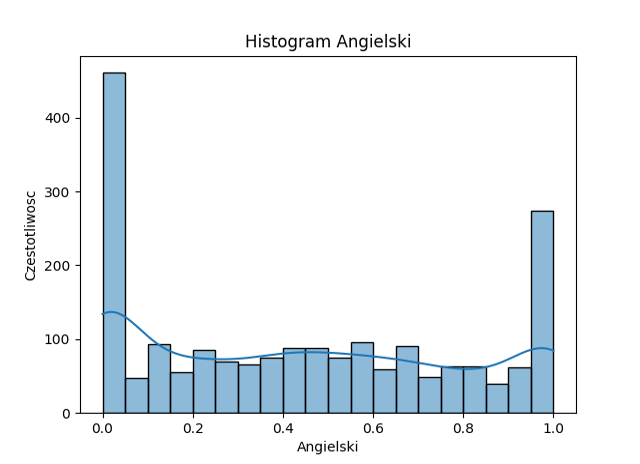
\includegraphics[width=\linewidth]{chapters/Images/hist_angielski.png}
            \cprotect\caption{Histogram umiejętności w kategorii Znajomość języka angielskiego\\ Źródło:\textit{ opracowanie własne}}
            \label{fig:hist_ang}
        \end{figure}

        \begin{enumerate}
            \item Podobnie jak w poprzednich kategoriach, najwyższe słupki dla kategorii znajomość języka angielskiego znajdują się przy wartościach $0$ (około $450$ pracowników) oraz $1$ (około $250$ pracowników). Około $1300$ pracowników ma umiejętności w przedziale od $0,1$ do $0,9$, a wartości blisko średniej posiada około $190$ pracowników. Krzywa gęstości potwierdza obserwacje dotyczącą rozkładu populacji na wykresie.
        \end{enumerate}
        
        \subsubsection{Umiejętności w kategorii Suma umiejętności}
        \begin{figure}[H]
            \centering
            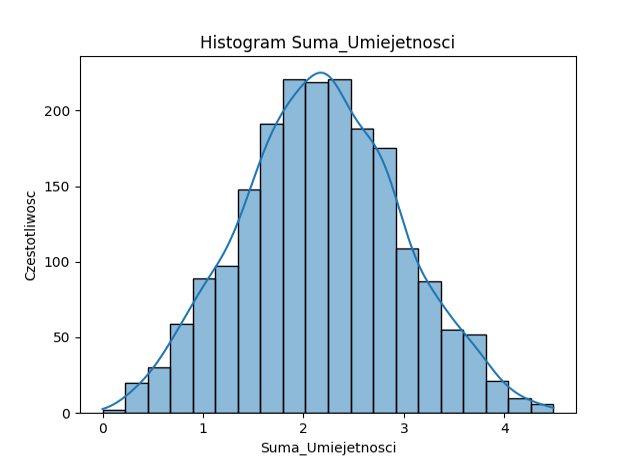
\includegraphics[width=\linewidth]{chapters/Images/hist_suma.png}
            \cprotect\caption{Histogram umiejętności w kategorii Suma umiejętności\\ Źródło:\textit{ opracowanie własne}}
            \label{fig:hist_suma}
        \end{figure}

        \begin{enumerate}
            \item Histogram dla kategorii Sumy umiejętności kształtem przypomina rozkład normalny (kształt dzwonu), co wskazuje na koncentrację pracowników około średniej sumy umiejętności, z minimalnymi przypadkami (około $80$ lub $0,04\%$ pracowników) ze skrajnie niską lub skrajnie wysoką sumą. Największa część tego zbioru (około $700$ lub $35\%$ pracowników) posiada sumę umiejętności zbliżoną do średniej. Odchylenie standardowe jest potwierdzone kształtem histogramu i potwierdza, że większość populacji ma wartość zbliżoną do średniej, a znaczna mniejszość posiada wartości skrajne. Minimum oraz maksimum również zostają odzwierciedlone na histogramie, gdyż widoczne są pojedyncze przypadki wartości minimalnych lub maksymalnych.
            \item Najwyższa częstotliwości w tej populacji występują w przedziale od $1,9$ do $2,5$, co dowodzi, że jest to najbardziej typowy poziom umiejętności w tej firmie. Częstotliwość spada niemal symetrycznie po obu stronach od średniej, co potwierdza podobieństwo do rozkładu normalnego.
            \item Łagodna krzywa gęstości również potwierdza podobieństwo do rozkładu normalnego i znikomość pracowników przy skrajnych wartościach. 
        \end{enumerate}

        \subsubsection{Umiejętności w kategorii Wynagrodzenie}
        \begin{figure}[H]
            \centering
            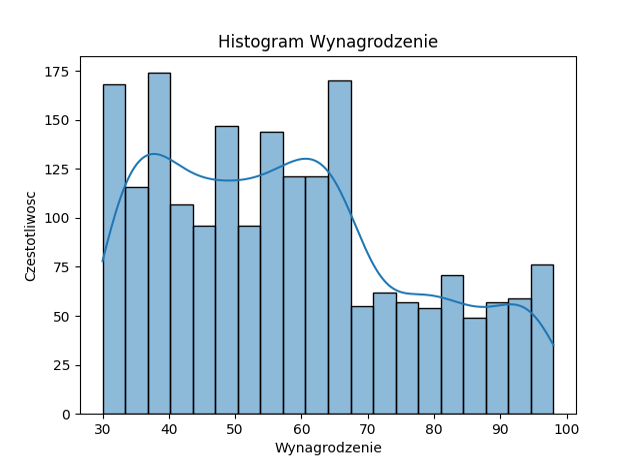
\includegraphics[width=\linewidth]{chapters/Images/hist_wynagrodzenie.png}
            \cprotect\caption{Histogram umiejętności w kategorii Wynagrodzenia\\ Źródło:\textit{ opracowanie własne}}
            \label{fig:hist_wynagrodzenie}
        \end{figure}

        \begin{enumerate}
            \item Histogram pokazuje wysokie rozproszenie kwoty wynagrodzenia na godzinę jaką otrzymują pracownicy firmy. Znaczna liczba populacji (około $460$) dostaje wynagrodzenie z przedziału $[30, 40]$ złotych/godzinę. Następnie widać wyraźny spadek dla przedziału $[40, 45]$ i nagły wzrost dla wartości około $50$. Po kolejnej drobnej fluktuacji, następuje kolejny wzrost dla drugiego wyraźnego szczytu w przedziale dla około $[55, 65]$, w którym częstotliwość wynosi około $575$. Pokazuje to, że znaczna część populacji (około $29\%$) dostaje wynagrodzenie między $55$, a $65$ złotych/godzinę co jest zgodne ze średnią. Dodatkowo odchylenie standardowe wskazuje na dużą zmienność wynagrodzenia w populacji, co jest dobrze uwidocznione na histogramie poprzez różnice w wysokościach słupków. Wyższe wynagrodzenia od $70$ do $100$ złotych na godzinie nie są już tak częste. Przedział jest trzy razy dłuższy od przedziału z najmniejszą płacą, a mieści się w nim tylko około $550$ pracowników.
            \item Krzywa gęstości pokazuje, że populacja jest głównie skoncentrowana w przedziale około $[30, 70]$ i stanowi to około $1450$ pracowników. Dodatkowo, krzywa posiada kilka szczytów co wskazuje na niejednolity rozkład. 
            \item Tendencyjnie krzywa gęstości osiąga najwyższe wartości w przedziałach $[30, 40]$ oraz $[50, 65]$ co stanowi o największej ilości pracowników zarabiających kwoty z tych przedziałów. Krzywa zalicza spadek przy wartościach większych od $70$ co dowodzi o małej części populacji zarabiającej kwoty powyżej $70$ złotych/godzinę. Długie ogony krzywej udowadniają małą liczbę pracowników zarabiające maksymalne i minimalne kwoty.
        \end{enumerate}
    
    \subsection{Macierz korelacji}\label{subsec:korelacja}
    \begin{figure}[H]
        \centering
        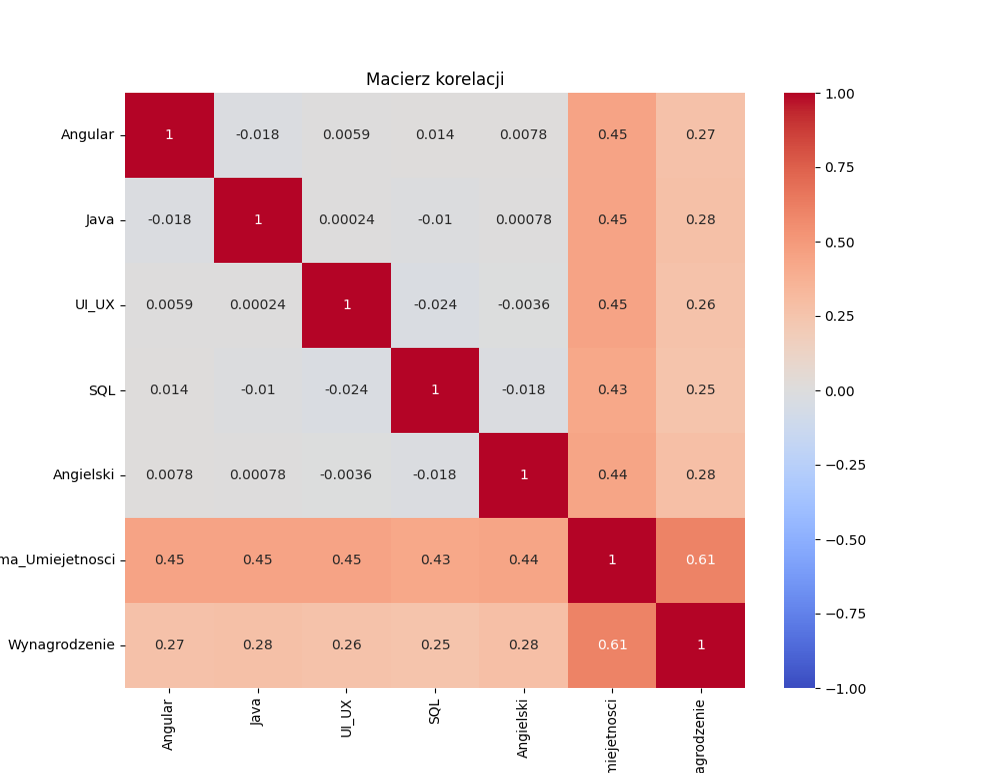
\includegraphics[width=\linewidth]{chapters/Images/korelacja.png}
        \cprotect\caption{Macierz korelacji danych\\ Źródło:\textit{ opracowanie własne}}
        \label{fig:korelacja}
    \end{figure}

    \par Do przedstawienia związków między poszczególnymi umiejętnościami, ich sumą oraz wynagrodzeniem wykorzystano macierz korelacji. Sprawdzenie, jak różne umiejętności oddziałują na siebie nawzajem oraz na sumę umiejętności i wynagrodzenie. Takie sprawdzenie pomoże ustalić, które z umiejętności mają największy wpływ na wynagrodzenie oraz jak rozwój poszczególnych umiejętności może wpłynąć na ogólny poziom kompetencji zespołu. Dzięki takiej analizie, menedżerowie mogą lepiej planować szkolenia, polityki wynagrodzeń oraz rekrutacje ze skutkiem zwiększenia efektywności i umiejętności w zespole.

    \par Związki między dwiema zmiennymi są opisane za pomocą liczb całkowitych z przedziału $[-1, 1]$, a wartości te oznaczają:
    \begin{enumerate}
        \item $1$ Oznacza dodatnią korelację; wysoka zależność między zmiennymi. W przypadku wzrostu jednej, druga też rośnie.
        \item $0$ Oznacza brak korelacji; zmienne są od siebie niezależne i nie oddziałują na siebie.
        \item $-1$ Oznacza ujemną korelację; wysoka zależność między zmiennymi. W przypadku wzrostu jednej, druga maleje.
    \end{enumerate}

    \par W przypadku korelacji między poszczególnymi umiejętnościami wartości są zawsze bliskie zeru, co oznacza, że np. posiadanie umiejętności w kategorii Angular, nie ma wpływu na poziom umiejętności SQL i na odwrót. Posiadanie umiejętności w jednej kategorii nie pomaga w zdobyciu umiejętności w innej kategorii, ale też nie utrudnia. 
    
    \par W kontekście sumy umiejętności, poszczególne umiejętności posiadają dodatnią korelację z sumą. Oznacza to, że wraz z wzrostem poszczególnych kategorii, pracownik będzie osiągać wyższą sumę umiejętności. Wpływ sumy jest też obserwowalny; gdy suma maleje, poszczególne umiejętności też maleją.

    \par Wynagrodzenie silnie koreluje z sumą umiejętności (a suma silnie koreluje z wynagrodzeniem). Pokazuje to, że wzrost wynagrodzenia bardzo często wiąże się z wysoką sumą umiejętności. Tak samo jak wysoka suma będzie wiązać się z wyższym wynagrodzeniem.

    \par Macierz korelacji pokazuje jaki wpływ mają na siebie poszczególne umiejętności oraz jak wpływają na wynagrodzenie i sumę. Dzięki takimi informacjom, menedżerowie mogą lepiej dostosować plan szkoleń w celu zwiększenia poziomu umiejętności zespołu i przewidzieć efekty jakie będzie to mieć na żądane wynagrodzenia. Dodatkowo, przy rekrutacjach będzie można ocenić jak wysokiego wynagrodzenia będzie oczekiwał pracownik w oparciu o jego umiejętności. Efektem takiego poglądu na relacje między zmiennymi będzie lepsze dostosowanie strategii przyznawania wynagrodzeń oraz dostosowanie szkoleń pod potrzeby zespołu. 
    
    \subsection{Wykres rozrzutu}\label{subsec:scatter}
    \begin{figure}[H]
        \centering
        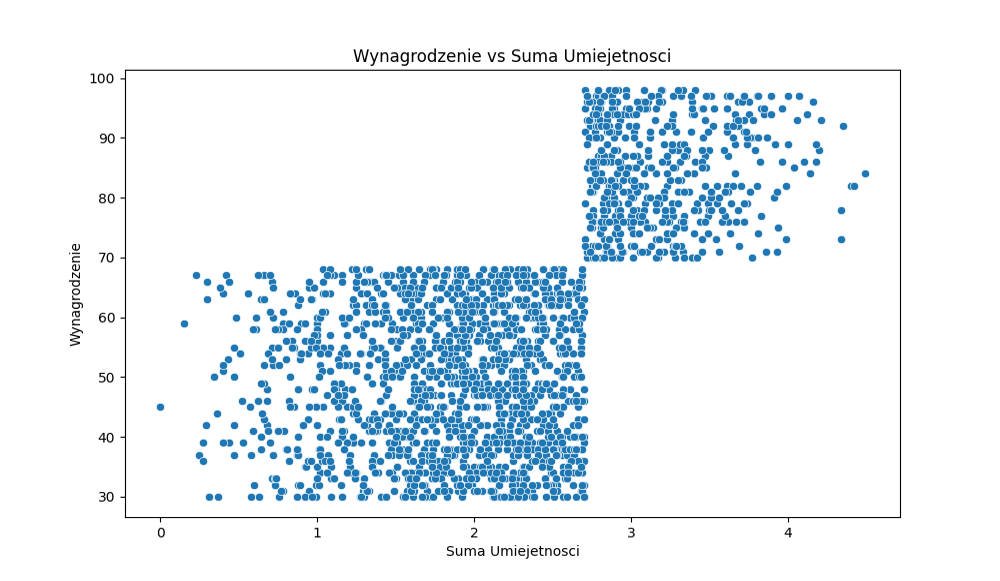
\includegraphics[width=\linewidth]{chapters/Images/rozrzut.png}
        \cprotect\caption{Wykres rozrzutu Wynagrodzenie vs Suma umiejętności\\ Źródło:\textit{ opracowanie własne}}
        \label{fig:scatter_plot}
    \end{figure}

    \par Do kolejnego etapu analizy wykorzystano wykres rozrzutu przedstawiający związek między danymi z kolumny Wynagrodzenie a danymi z kolumny Suma umiejętności. Oś X reprezentuje zakres sumy umiejętności, a analogicznie oś Y reprezentuje zakres wynagrodzeń. Punkty na wykresie oznaczają poszczególnego pracownika z populacji.

    \par Wykres jest bardzo widocznie podzielony na dwa wyraźne klastry punktów. Pierwszy i większy klaster obejmuje na osi X obszar od $0$ do około $2,7$ i na osi Y od $30$ do około $70$. Reprezentuje on część populacji, posiadającą sumę umiejętności poniżej $3$, która w efekcie zarabia w przedziale około $[30, 70]$. W tym klastrze, wynagrodzenie nie wykazuje bardzo silnej zależności od sumy umiejętności, co oznacza że nawet pracownicy z niską sumą zarabiają kwoty w górnej granicy przedziału. 

    \par W drugim klastrze znajduje się część populacji o sumie umiejętności w przedziale od około $2,7$ do $5$ i o wynagrodzeniu z przedziału około $[70, 100]$. Ten klaster pokazuje, że wyższy poziom umiejętności wiąże się z wyższym wynagrodzeniem. Można zauważyć, że nawet minimalny wzrost poziomu umiejętności ponad dolną granice tego przedziału powoduje spory wzrost wynagrodzenia. Dzieje się tak z powodu w jaki zostały wygenerowane dane; pracownicy, których suma umiejętności jest większa od trzeciego kwartyla, otrzymują losowe wynagrodzenie z przedziału $[70, 99]$. 

    \par Wykres ten można również zidentyfikować jako wykres:
    \begin{enumerate}
        \item Z silną istotnością zależności. Oznacza to, że zmienne z osi X i Y silnie na siebie oddziałują.
        \item Z liniowym rodzajem korelacji. Wraz z wzrostem wartości na osi X, wzrastają wartości na osi Y.
        \item Nieposiadający wartości odstających.
    \end{enumerate}

    \par Informacje z takiego wykresu mogą posłużyć menedżerom do opracowania lepszej polityki rozwojowej dla pracowników, która będzie nagradzać wyższe umiejętności lepszym wynagrodzeniem. Szczególnie po przekroczeniu progu (około $2,7$) wynagrodzenie zostaje znacznie zwiększone, co może silnie motywować pracowników do rozwoju swoich umiejętności. Pomoże to również w ocenie sprawiedliwości przyznawanych wynagrodzeń, mogą zdarzać się wypadki, gdy ktoś mniej uzdolniony zarabia kwotę z górnej części przedziału, a pracownik z wyższymi umiejętnościami zarabia rażąco mniej.


%<<<<<<<<<<<<<<<<<<<<<<<<<<<<<<<<<<<<<<<< ANALIZA WYNIKÓW >>>>>>>>>>>>>>>>>>>>>>>>>>>>>>>>>>>>>>>>>>>>>>>>>>>>>    
    \subsection{Interpretacja analizy wyników optymalizacji}\label{subsec:analiza_optimal}
    \par Przeanalizowane wyniki optymalizacji przez skrypt \verb|optimizer.py| zostały przeanalizowane przez \verb|analyzer.py|. Plik posiada nazwę jaką nadał mu użytkownik w momencie uruchamiania skryptu analizującego. Dane z analizy zostały podzielone na dwa arkusze. Pierwszy - \verb|Statystyki| zawiera tabele z podstawową analizą statystyczną w formie tabeli i drugi - \verb|Wykresy| zawiera histogramy, macierz korelacji i wykres rozrzutu.

    \subsection{Analiza porównawcza danych z tabeli}
    \par Tabela przedstawiona na rysunku \ref{fig:tabela_analiza_wybrani} przedstawia zestawienie statystyk obliczonych przez skrypt \verb|analyzer.py|. Struktura danych w tabeli została już opisana w przypadku populacji przy omawianiu tabeli \figrefnote{fig:tabela_analiza}.

    \begin{figure}[H]
        \centering
        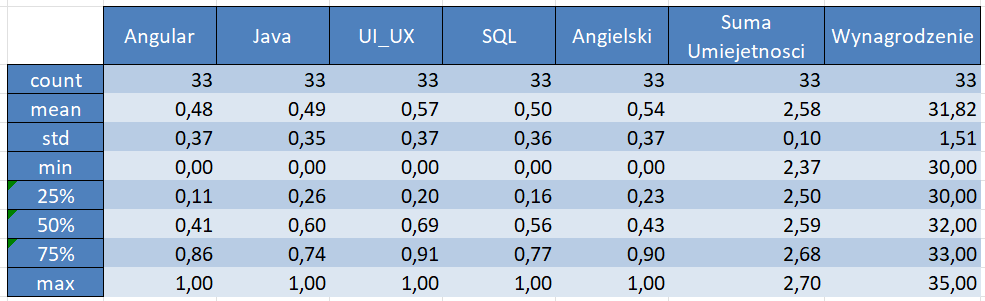
\includegraphics[width=\linewidth]{chapters/Images/analiza_tabela_wybrani.png}
        \cprotect\caption{Tabela wybranego zespołu projektowego po analizie\\ Źródło:\textit{ opracowanie własne}}
        \label{fig:tabela_analiza_wybrani}
    \end{figure}

    \par Z tak wygenerowanej tabeli można wyciągnąć następujące wnioski:
    \begin{description}
        \item[Rozmiar populacji\label{itm:count_2}]  - Pokazuje rozmiar populacji i potwierdza, że analiza została przeprowadzona na pełnym zestawie danych, otrzymanym ze skryptu \verb|optimizer.py| pracującego z zestawem danych z pliku \verb|pracownicy.csv|.
        
        \item[Średnia\label{itm:mean_2}] - Średnia z każdej umiejętności dla wybranych pracowników wynosi od $0,48$ do $0,57$. Te wartości są wyższe dla każdej kategorii w porównaniu do populacji. Podobnie w przypadku średniej sumy umiejętności, optymalny zespół posiada wyższą ogólną średnią niż populacja pracowników. Dodatkowo, wybrany zespół oczekuje średnio mniejszego wynagrodzenia, niż populacja w firmie. Wybrany zespół jest nie tylko lepszy pod kątem umiejętności, ale też wymaga mniejszych funduszy, co jest korzystne dla firmy.
        
        \item[Odchylenie standardowe\label{itm:std_2}] - Odchylenie std. dla grupy wybranych pracowników w poszczególnych umiejętnościach jest na podobnym poziomie, co u populacji. Jednak w przypadku sumy umiejętności i wynagrodzenia jest znacznie niższe ($8$ razy mniejsze dla sumy, $12$ razy mniejsze dla wynagrodzenia), co oznacza, że pracownicy w optymalnym zespole mają podobny poziom umiejętności oraz oczekują podobnego wynagrodzenia.
        
        \item[Minimum\label{itm:min_2}] - Podobnie jak w przypadku populacji, wartości poszczególnych umiejętności osiągają $0$, jednak minimum sumy umiejętności wynoszące $2,37$ jest znacznie wyższe od populacji co oznacza dużą poprawę nad minimum populacji. Minimalne wynagrodzenie wynoszące $30$ jest również takie samo jak w populacji.
        
        \item[Maksimum\label{itm:max_2}] - Dla maksimum poszczególnych kategorii, dane wynoszą tyle samo co w przypadku populacji. Jednak maksimum łącznej sumy umiejętności jest znacznie niższe niż w przypadku populacji o dokładnie $1,79$. Maksimum wynagrodzenia w optymalnym zespole wynosi $35$ złotych na godzinę.
        
        \item[Kwartyle 25\%, 50\% i 75\%\label{itm:kwartyl_2}] - Kwartyle dla optymalnego zespołu są wyższe dla prawie każdej kategorii poza wynagrodzeniem, co oznacza, że optymalny zespół posiada generalnie wyższe umiejętności i wymaga mniejszego wynagrodzenia.
            \begin{itemize}
                \item Każdy kwartyl poszczególnych umiejętności oraz sumy umiejętności jest wyższy od populacji. W kwartylu pierwszym różnice sięgają od $0,8$ do $0,19$ punktów. W drugim od $0,3$ do $0,29$ punktów, a w kwartylu trzecim jedynie umiejętności z kategorii \verb|Java| są na poziomie niższym o $0,03$. Największa różnica w kwartylu trzecim jest w kategoriach \verb|Angular, UI/UX| oraz w \verb|Angielski| i wynosi $0,15$. Suma umiejętności w trzecim kwartylu jest niewiele niższa o $0,03$.
                \item Wynagrodzenie pozostaje niższe w trzecim i drugim kwartylu kolejno różniące się o $37$ złotych i $24$ złote.
            \end{itemize}
        
    \end{description}
    
    \par Porównanie wyników z analizy populacji oraz analizy optymalnego zespołu pokazuje, że mimo ogólnie lepszych statystyk, optymalny zespół może nie posiadać pracowników z bardzo wysoką generalną ekspertyzą. Warunek utrzymania niskiego kosztu pozwolił dobrać pracowników, nieoczekujących wysokiego wynagrodzenia, ale kosztem eksperckich umiejętności w zespole.
    
    \subsection{Histogramy}
    \par Histogramy przedstawiają częstotliwość występowania pracowników o danych poziomach umiejętności, wynagrodzenia czy sumy umiejętności. Podobne wykresy zostały opisane wcześniej i następująca analiza będzie porównywać wyniki do analizy przeprowadzonej w sekcji \refnote{subsec:histogramy}.
    
        \subsubsection{Umiejętności w kategorii Angular optymalnego zespołu}
        \begin{figure}[H]
            \centering
            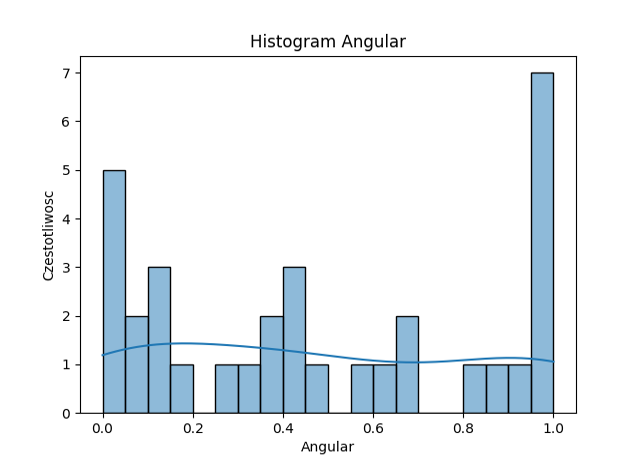
\includegraphics[width=\linewidth]{chapters/Images/hist_angular_optimal.png}
            \cprotect\caption{Histogram umiejętności w kategorii Angular dla optymalnego zespołu\\ Źródło:\textit{ opracowanie własne}}
            \label{fig:hist_angular_optimal}
        \end{figure}

        \begin{enumerate}
            \item Występowanie najwyższych słupków przy wartościach $0$ i $1$ jest podobne do tego przy populacji, jednak w optymalnym zespole $21\%$ pracowników posiada pełną ekspertyzę w tej kategorii, a tylko $15\%$ nie posiada żadnej wiedzy.
            \item Rozkład poziomu umiejętności $[0,1; 0,9]$ jest bardziej zróżnicowany niż ten populacji. Widoczne są wyraźne szczyty przy $0,2$, $0,4$ i $0,6$ co sugeruje, że optymalny zespół posiada bardziej zróżnicowany poziom umiejętności, ale generalnie na wyższym poziomie. Ponad połowa wybranego zespołu ($18$) posiada umiejętności wyższe niż średnia populacji.
            \item Krzywa gęstości potwierdza obserwacje z poprzedniego punktu, ale jest bardziej płaska niż dla populacji, potwierdzając większe zróżnicowanie w poziomie umiejętności.
        \end{enumerate}
        
        \par Z histogramu można wywnioskować, że optymalny zespół posiada generalnie wyższy poziom umiejętności w kategorii Angular od populacji. Nie oznacza to jednak, że każdy członek zespołu posiada ekspertyzę w tym zakresie, gdyż w zespole znajdują się też pracownicy bez żadnej wiedzy w danym temacie. Można zakładać, że optymalizacja przyniosła pożądane efekty.
        
        \subsubsection{Umiejętności w kategorii Java optymalnego zespołu}
        \begin{figure}[H]
            \centering
            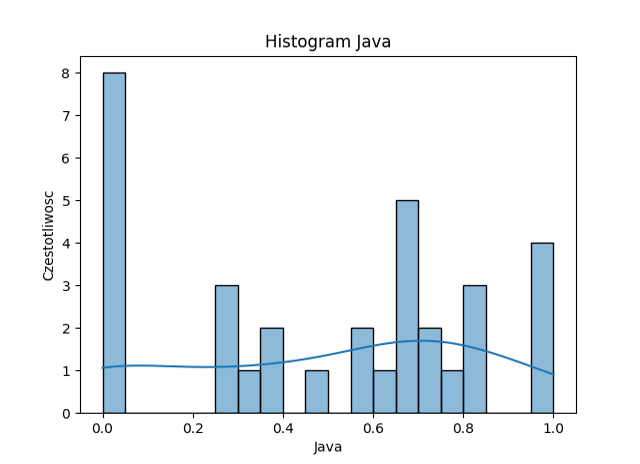
\includegraphics[width=\linewidth]{chapters/Images/hist_java_optimal.png}
            \cprotect\caption{Histogram umiejętności w kategorii Java dla optymalnego zespołu\\ Źródło:\textit{ opracowanie własne}}
            \label{fig:hist_java_optimal}
        \end{figure}

        \begin{enumerate}
            \item Najwyższe słupki na histogramie umiejętności z kategorii Java znajdują się przy punktach $0$, $1$ oraz około przedziału $[6,5; 0,7]$. Umiejętności w tej kategorii nie posiada ośmiu pracowników, natomiast ekspertyzę powyżej średniej optymalnego zespołu posiada $18$ pracowników, w tym $4$ posiada wiedzę na poziomie eksperta. Jest to znaczy wyższy poziom wiedzy od średniej populacji.
            \item Krzywa gęstości jest generalnie płaska, ze szczytami około $0,6$ oraz $1$. Taka krzywa, może sugerować sporą różnorodność w zespole w tej kategorii i ogólnie wyższy poziom umiejętności niż dla populacji.
        \end{enumerate}

        \par Umiejętności z kategorii Java są generalnie wyższe od średniej populacji, ale nie brakuje zróżnicowania w zespole. Znajdują się w nim i pracownicy, których można określać ekspertami w tej kategorii oraz pracownicy z wiedzą znikomą. Widać zamierzone efekty optymalizacji.
        
        \subsubsection{Umiejętności w kategorii UI/UX optymalnego zespołu}
        \begin{figure}[H]
            \centering
            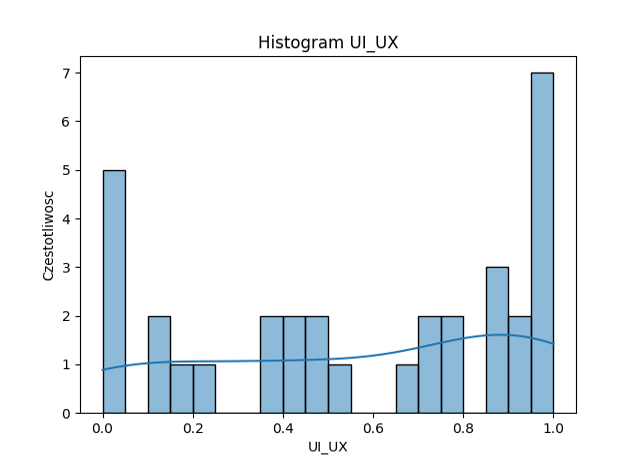
\includegraphics[width=\linewidth]{chapters/Images/hist_uiux_optimal.png}
            \cprotect\caption{Histogram umiejętności w kategorii UI/UX dla optymalnego zespołu\\ Źródło:\textit{ opracowanie własne}}
            \label{fig:hist_uiux_optimal}
        \end{figure}

        \begin{enumerate}
        \item Histogram kategorii UI/UX wykazuje, że poziom umiejętności $1$ oraz $0$ osiągnęło kolejno $7$ oraz $5$ pracowników. Ponownie pojawia się przewaga pracowników na poziomie eksperckim, co nie było obecne w populacji, w której nad ekspertami, przeważały osoby z brakiem jakiejkolwiek wiedzy w danej kategorii. Poza dwoma głównymi szczytami, na wykresie nie przebijają się inne znaczące szczyty. Ogólny rozkład w przedziale $[0,1; 0,9]$ jest równomierny, jednak ponad połowa wybranych pracowników ($18$) ma umiejętności wyższe od średniej populacji.
        \item Krzywa gęstości jest generalnie płaska, z lekkim wzrostem ku końcowi przedziału, co sugeruje równomierne rozłożenie umiejętności oraz przeważającą liczbę pracowników o poziomie wyższym od $0,5$ i średniej populacji.
        \end{enumerate}

        \par Zróżnicowanie umiejętności w kategorii UI/UX i przewaga umiejętności na poziomie wyższym od średniej populacji potwierdza działanie modelu, który przy niskim koszcie dobrał wysoce wykwalifikowany zespół.
        
        \subsubsection{Umiejętności w kategorii SQL optymalnego zespołu}
        \begin{figure}[H]
            \centering
            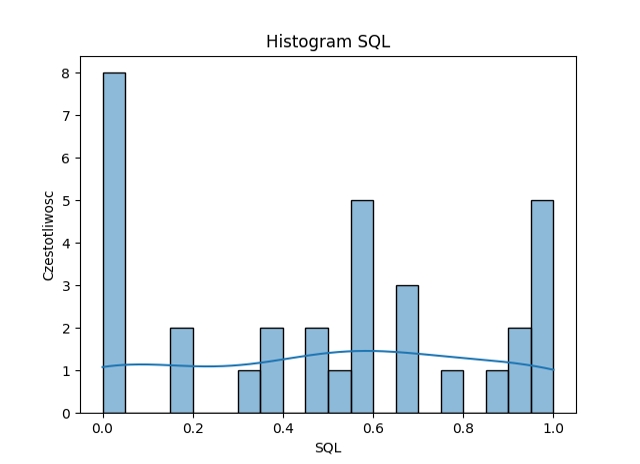
\includegraphics[width=\linewidth]{chapters/Images/hist_sql_optimal.png}
            \cprotect\caption{Histogram umiejętności w kategorii SQL dla optymalnego zespołu\\ Źródło:\textit{ opracowanie własne}}
            \label{fig:hist_sql_optimal}
        \end{figure}

        \begin{enumerate}
            \item Najwyższe słupki są dla wartości $0$, $1$ oraz $0,6$ i stanowią kolejno $8$. $5$ i $5$ pracowników z optymalnego zespołu. Mimo dużego odsetku osób bez żadnej wiedzy (około $24\%$) zespół nadal posiada wysoki poziom wiedzy w zakresie SQL. Umiejętności ponad średnią populacji posiada $17$ pracowników co stanowi ponad połowę tego zespołu. Znaczna część tego zespołu posiada odpowiedni poziom ekspertyzy, żeby z powodzeniem wykonać powierzone zadania.
            \item Krzywa gęstości potwierdza obserwacje i wskazuje na duże zróżnicowanie w zespole, pojawiają się w nim zarówno osoby bez umiejętności, eksperci oraz osoby z umiejętnościami wyższymi niż średnie.
        \end{enumerate}

        \par Przeważające umiejętności na poziomie wyższym od średniej populacji sugerują, że i w tej kategorii model dokonał poprawnej optymalizacji.
        
        \subsubsection{Umiejętności w kategorii Znajomość języka angielskiego optymalnego zespołu}
        \begin{figure}[H]
            \centering
            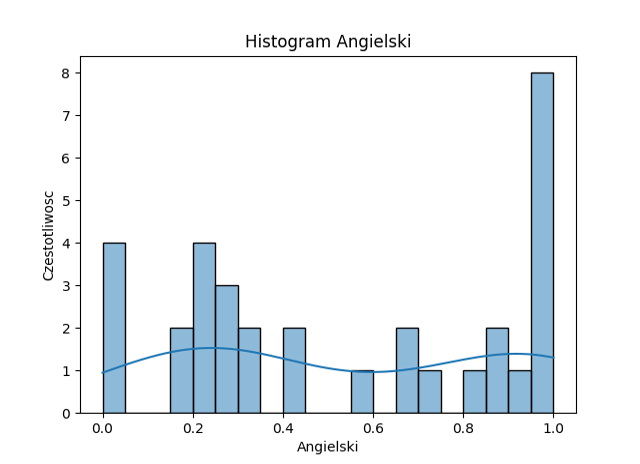
\includegraphics[width=\linewidth]{chapters/Images/hist_ang_optimal.png}
            \cprotect\caption{Histogram umiejętności w kategorii Znajomość języka angielskiego dla optymalnego zespołu\\ Źródło:\textit{ opracowanie własne}}
            \label{fig:hist_ang_optimal}
        \end{figure}

        \begin{enumerate}
            \item Dwa razy wyższy słupek symbolizujący osoby z perfekcyjną znajomością języka angielskiego, niż tego symbolizującego osoby bez żadnej wiedzy. Mimo tego, $17$ pracowników zna język angielski na poziomie niższym od średniej populacji, co nie jest zadowalające.
            \item Krzywa wskazuje na zrównoważony rozkład umiejętności pośród pracowników, ze szczytem w okolicach przedziału $[0,2; 0,3]$ i w okolicach $[0,9; 1]$.
        \end{enumerate}

        \par Mimo niezadowalającej przewagi pracowników z poziomem języka angielskiego niższym niż średnia populacji, nie jest to krytyczna umiejętność, która nie pozwala zespołowi spełnić zadania.
        
        \subsubsection{Umiejętności w kategorii Suma umiejętności optymalnego zespołu}
        \begin{figure}[H]
            \centering
            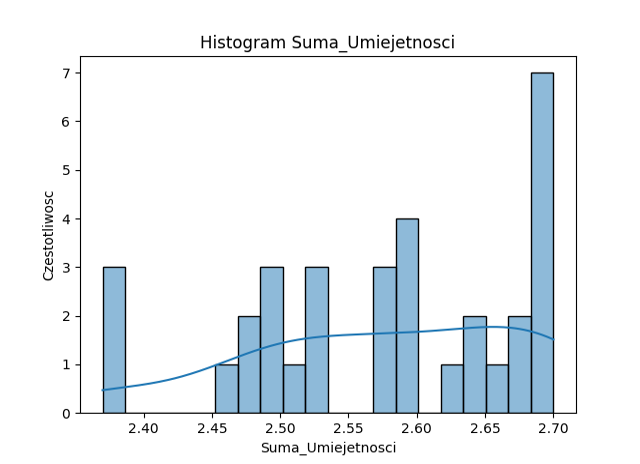
\includegraphics[width=\linewidth]{chapters/Images/hist_suma_optimal.png}
            \cprotect\caption{Histogram umiejętności w kategorii Suma umiejętności dla optymalnego zespołu\\ Źródło:\textit{ opracowanie własne}}
            \label{fig:hist_suma_optimal}
        \end{figure}

        \begin{enumerate}
            \item Najwyższym słupkiem jest ten z poziomem sumy umiejętności w okolicach $2,70$, co wskazuje na ogólnie wysoki poziom sumarycznych umiejętności zespołu. Tych siedmiu pracowników niemal posiada tak wysoka sumę umiejętności jak kwartyl trzeci populacji i znacznie przewyższa średnią populacji o $0,53$ punktów.
            \item Krzywa sugeruje znaczący wzrost sumy umiejętności od około $2,45$, co stanowi o dużej gęstości pracowników, których sumaryczne umiejętności przewyższają nad średni populacji o przynajmniej $0,25$ i więcej.
        \end{enumerate}

        \par Suma umiejętności jest większa od średniej populacji nawet w swoim minimum, co oznacza dużą poprawę poziomu umiejętności nad całą populacją. Model dokonał poprawnych wyborów co do członków zespołu w trakcie optymalizacji pod minimalny poziom umiejętności.

        \subsubsection{Umiejętności w kategorii Wynagrodzenie optymalnego zespołu}
        \begin{figure}[H]
            \centering
            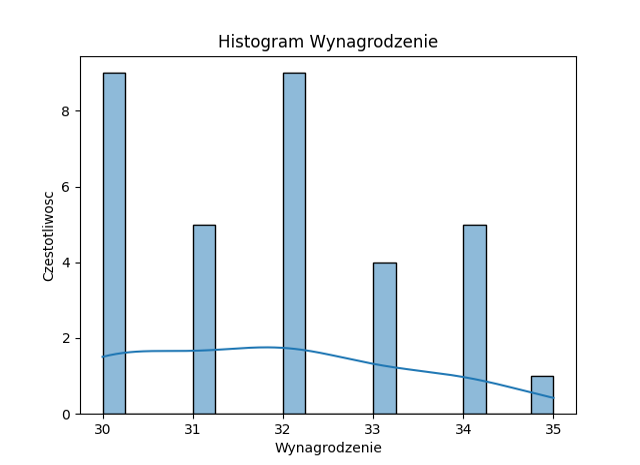
\includegraphics[width=\linewidth]{chapters/Images/hist_wynagrodzenie_optimal.png}
            \cprotect\caption{Histogram umiejętności w kategorii Wynagrodzenia dla optymalnego zespołu\\ Źródło:\textit{ opracowanie własne}}
            \label{fig:hist_wynagrodzenie_optimal}
        \end{figure}

        \begin{enumerate}
            \item Najwyższe słupki znajdują się na wartościach $30$ oraz $32$ (złotych na godzinę). Oznacza to, że w wybranym zespole prawie połowa wybranych ($16$ lub $48\%$) pracowników zarabia stawkę minimalną pod kątem populacji lub bliską minimalnej. Jest tylko jeden pracownik, który zarabia najwięcej a jego zarobki nie przekraczają średniej populacji.
            \item Krzywa gęstości wskazuje na zagęszczenie pracowników w przedziale od $30$ do $32$ z następującym spadkiem. Można z tego wywnioskować, że wynagrodzenie w tym zespole jest wyjątkowo niskie w stosunku do danych z populacji.
        \end{enumerate}
        
        \par Dane z histogramu kategorii Wynagrodzenie ponownie potwierdzają działanie i sukces modelu w optymalizacji zespołu projektowego pod ograniczeniem budżetu oraz umiejętności zespołu.
    
    \subsection{Macierz korelacji}
    \begin{figure}[H]
        \centering
        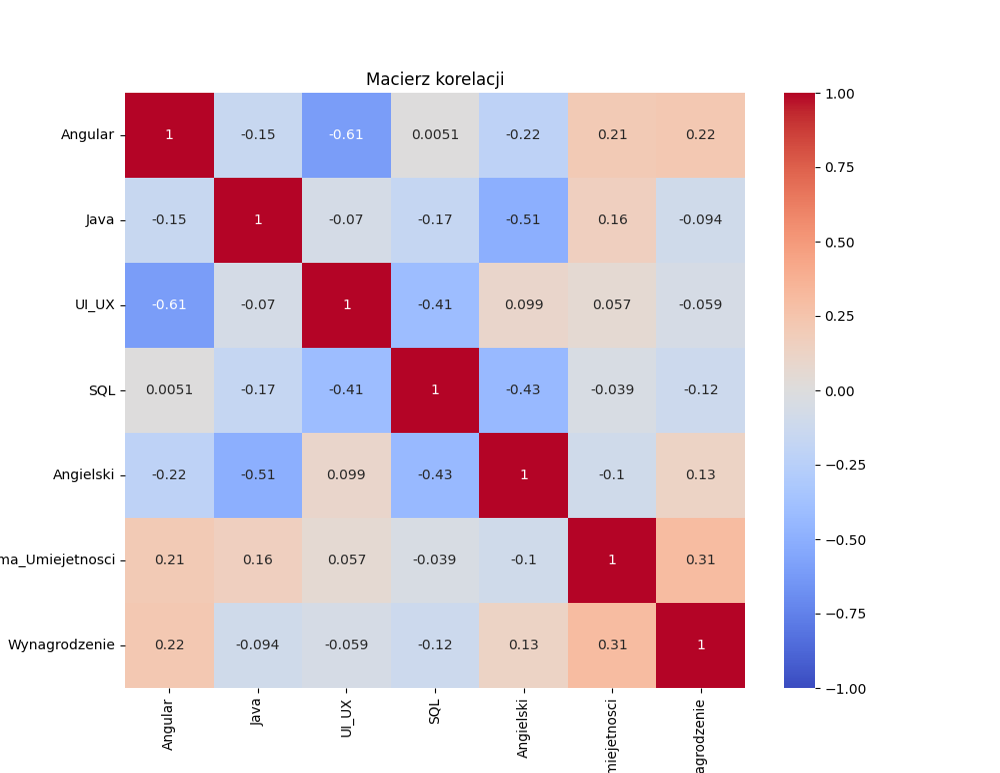
\includegraphics[width=\linewidth]{chapters/Images/korelacja_optimal.png}
        \cprotect\caption{Macierz korelacji danych\\ Źródło:\textit{ opracowanie własne}}
        \label{fig:korelacja_optimal}
    \end{figure}

    \par Ponownie wykorzystano macierz korelacji do przedstawienia związków między poszczególnymi umiejętnościami, ich sumą, a wynagrodzeniem. Analiza macierzy ma pomóc w ustaleniu czy dobór optymalnego zespołu jest skuteczniejszy dzięki niektórym korelacjom między umiejętnościami. Znaczenie wartości na macierzy zostało opisane w sekcji \refnote{subsec:korelacja}.

    \par W przypadku korelacji między poszczególnymi umiejętnościami wartości są zawsze bliskie zeru lub ujemne, a co za tym idzie nie oddziałują na siebie albo oddziałują na siebie negatywnie. W praktyce oznacza to, że posiadanie umiejętności np. z kategorii Angular nie oddziałuje na umiejętności z kategorii SQL (korelacja na poziomie $0,0051$) i na odwrót. Negatywna korelacja między kategorią Angular i kategorią UI/UX oznacza, że posiadanie wysokich umiejętności w jednym wiąże się z posiadaniem niskich umiejętności w drugim (korelacja na poziomie $-0,61$). W macierzy korelacji populacji, poszczególne umiejętności nie oddziaływały na siebie prawie w ogóle.
    
    \par W kontekście sumy umiejętności, poszczególne umiejętności posiadają głównie dodatnią lub bliską zeru korelację z sumą. Wraz ze wzrostem poziomu umiejętności, ekspertyza w innych kategoriach wzrasta lub pozostaje bez zmian. Wskazuje to na wzrost sumy wraz z ze wzrostem poszczególnych umiejętności, ale także i spadek. W przypadku populacji, suma silnie korelowała z każdą z kategorii umiejętności co oznaczało gwałtowne wzrosty oraz spadki.

    \par Wynagrodzenie silnie koreluje z sumą umiejętności, ale nie tak mocno jak w przypadku populacji. W populacji pracowników, wyższa suma umiejętności w wielu przypadkach wiązała się z wysokim wynagrodzeniem, w przeciwieństwie do optymalnego zespołu. Pokazuje to, że mimo wzrostu sumy umiejętności, w optymalnym zespole zmiany w oczekiwanym wynagrodzeniu nie są tak gwałtowne.

    \par Analiza porównawcza macierzy korelacji optymalnego zespołu w porównaniu z macierzą populacji ukazuje pewne tendencje w populacji, które zostały uwidocznione dopiero po ich zestawieniu. Mianowicie w populacji wyższy poziom umiejętności był silnie związanym ze wzrostem wynagrodzenia, gdzie w optymalnym zespole wymagane podwyżki są stosunkowo niskie. Również w populacji nie był widoczny wpływ posiadania wiedzy z jednej kategorii na inne. W przypadku optymalnego zespołu te wpływy są nieco bardziej widoczne i można zauważyć przeważnie negatywne oddziaływanie umiejętności na siebie.
    
    \subsection{Wykres rozrzutu}
    \begin{figure}[H]
        \centering
        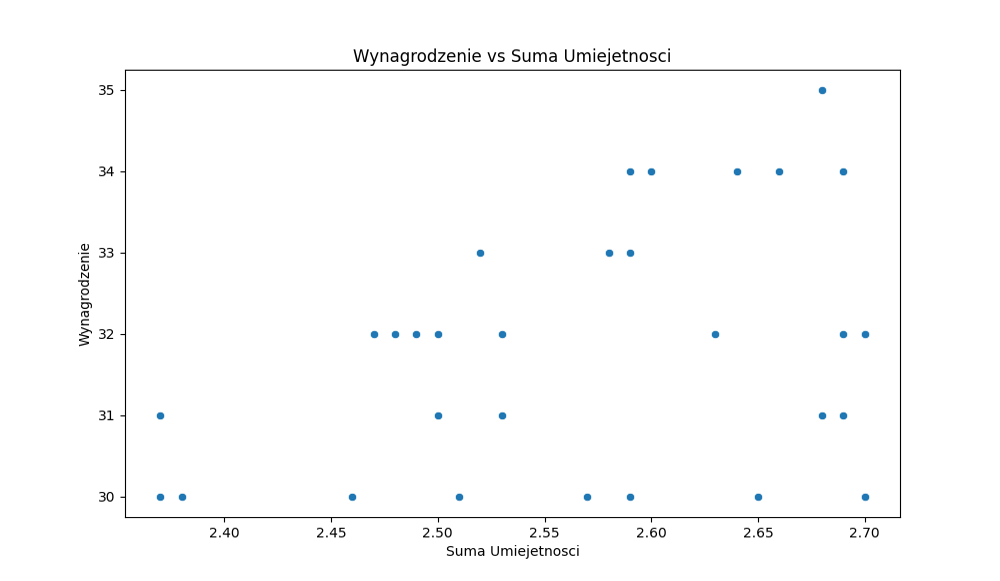
\includegraphics[width=\linewidth]{chapters/Images/rozrzut_optimal.png}
        \cprotect\caption{Wykres rozrzutu Wynagrodzenie vs Suma umiejętności\\ Źródło:\textit{ opracowanie własne}}
        \label{fig:scatter_plot_optimal}
    \end{figure}

    \par Ostatnia część analizy bazuje na wykresie rozrzutu przedstawiającego stosunek sumy umiejętności do wynagrodzenia w optymalnym zespole. Oś X przedstawia sumę umiejętności a oś Y wynagrodzenie. Punkty na wykresie to każdy z pracowników w optymalnym zespole.

    \par Wykres został bardzo widocznie podzielony prawie "na pół". Jedyny klaster na wykresie obejmuje obszar na osi X od $2,4$ do $2,7$ i na osi Y obszar od $30$ do $35$. Nie jest widoczna silna zależność między sumą umiejętności, a wynagrodzeniem, co sugeruje, że wybrani pracownicy posiadają wysoką sumę umiejętności, której stosunek do wynagrodzenia jest minimalny. Nie zaobserwowano również żadnej tendencji wskazującej na znaczy wzrost wynagrodzenia względem sumy umiejętności. W zestawieniu z wykresem rozrzutu populacji, można stwierdzić że pracownicy optymalnego zespołu "mieszczą się" w klastrze pierwszy wykresu rozrzutu populacji (Wykres rozrzutu populacji \figrefnote{fig:scatter_plot}).

    \par Wykres ten można również zidentyfikować jako wykres:
    \begin{enumerate}
        \item Z umiarkowaną istotnością zależności. Oznacza to, że zmienne z osi X i Y oddziałują na siebie, ale nie w silny sposób.
        \item Z liniowym rodzajem korelacji. Wraz z wzrostem wartości na osi X, wzrastają wartości na osi Y.
        \item Nieposiadający wartości odstających. Punkty są skoncentrowane w ramach jednego klastra i można stwierdzić brak wartości odstających.
    \end{enumerate}

    \par Informacje z takiego wykresu wskazują na skuteczność modelu optymalizacyjnego przy wyborze optymalnego zespołu projektowego. Model ograniczył swoje wybory do pracowników o wysokiej sumie umiejętności i niskich oczekiwaniach finansowych. Jednorodność klastra może sugerować, większe podobieństwo między pracownikami pod względem umiejętności.

\clearpage
\addcontentsline{toc}{chapter}{Podsumowanie}
\chapter*{Podsumowanie}
\par Celem oraz hipotezami\parrefnote{par:hipotezy} tej pracy dyplomowej było opracowanie, implementacja i analiza modelu optymalizacyjnego przeznaczonego do efektywnego zarządzania zasobami w firmie z sektora IT. Jako cel modelu ustalono minimalizację kosztów wynagrodzeń pracowników zespołu projektowego w firmie oraz dodano ograniczenia, których model musiał przestrzegać. Danymi wejściowymi dla modelu oraz badania, był syntetycznie generowany zestaw danych o pracownikach, zawierających różne metryki. Następnie zostało przeprowadzone badanie mające udowodnić użyteczność i poprawność modelu oraz rozumowania prowadzącego do jego powstania. Przeprowadzone badanie, polegające na analizie statystycznej wyników optymalizacji, dowiodło o skuteczności modelu, a wyniki badania zostały omówione w sekcji \refnote{sec:analiza}. Skutecznie przeprowadzone badanie potwierdza hipotezy oraz odpowiada twierdząco na pytanie: czy jest możliwym stworzenie, zaimplementowanie i przeanalizowanie w języku programowania Python modelu matematycznego, który stworzy optymalny zespół przy zadanych ograniczeniach.

\section*{Omówienia przeprowadzonego badania}
\par Praktyczna część pracy została poświęcona na studium przypadku opartego o zadanie optymalizacyjne (sekcja \refnote{sec:studium}). Problemem optymalizacyjnym, było utworzenie optymalnego zespołu pracowników, którzy w określonym zakresie czasu wykonają dany projekt przy jak najniższym koszcie wynagrodzeń oraz będą posiadać wysoki poziom umiejętności.
\par Przedstawiony problem wymagał zestawu danych, na który można by przeprowadzić optymalizację. W celu symulacji rzeczywistych warunków rynkowych, wygenerowano syntetyczne losowe dane w oparciu o rozkład normalny, w sposób opisany w sekcji \refnote{sec:kod_generator}. 
\par Optymalizacja została przeprowadzona za pomocą skryptu \verb|optimizer.py| (sekcja \refnote{subsec:optimizer_implementacja}) na wcześniej wygenerowanym zestawie danych. Otrzymane z niej wyniki zostały następnie poddane analizie statystycznej przez skrypt \verb|analyzer.py|, a otrzymane rezultaty i implementacja skryptu zostały omówione w sekcji \refnote{sec:analiza}. 
\par Przeanalizowane zostały dane wejściowe (populacja pracowników) oraz optymalny zespół stworzony przez model. Analiza wyników potwierdziła skuteczność modelu optymalizacyjnego. Optymalnie wybrany zespół posiadał wysoki poziom umiejętności (wyższy od poziomu populacji, wykres \figrefnote{fig:hist_suma_optimal}) oraz pracownicy oczekują dużo niższych wynagrodzeń niż średni pracownik w populacji (wykres \figrefnote{fig:hist_wynagrodzenie_optimal}). 
\par Takie efekty były oczekiwane od modelu, który z sukcesem dowiódł swojego działania tworząc optymalny, tani w finansowaniu i dobrze wyszkolony zespół. Z wyników badań można również wyciągnąć kilka innych wniosków, które zostały omówione w następnej sekcji.

\section*{Główne wnioski z pracy}
\par Przeprowadzone badanie przede wszystkim dowodzi o skuteczności utworzonego modelu. Tak utworzony model, dostosowany do potrzeb, mógłby również zostać zastosowany w rzeczywistym scenariuszu. Odpowiednio przygotowane dane wejściowe jak i dobrze określona funkcja celu wraz z ograniczeniami, mogą znacząco przyczynić się do poprawy procesu zarządzania zespołami projektowymi i nie tylko. 

\par Z wyników analizy, menedżerowie mogą dowiedzieć się o wpływie jaki ogólny poziom umiejętności ma na oczekiwania finansowe pracownika. Pozwala to na lepsze przygotowanie polityki wynagrodzeń oraz pomaga w przewidywaniu, jakich stawek będą oczekiwać pracownicy po zdobyciu nowych, znaczących umiejętności.

\par Dodatkowo menedżerowie mogą zauważyć, że do optymalnego zespołu nie został wybrany żaden z pracowników, którego suma umiejętności była bliska maksimum (patrz sekcja \refnote{subsec:tabela_populacja}, paragraf o \parrefnote{itm:max}). Pokazuje to, że do utworzenia optymalnego zespołu ze sztywnymi ograniczeniami budżetowymi, lepiej wybierać pracowników o mniejszej ekspertyzie (nadal powyżej średniej populacji \refnote{fig:hist_suma_optimal}) oczekujących niższego wynagrodzenia.


% \newpage
% \printbibliography[title={Źródła internetowe},notkeyword={external}]


% \newpage
% \printbibliography[title={Literatura},notkeyword={external}]

% \lstlistoflistings
\clearpage

\addcontentsline{toc}{chapter}{Bibliografia}
\printbibliography

\newpage
\addcontentsline{toc}{chapter}{Spis rysunków}
\listoffigures

\newpage
\addcontentsline{toc}{chapter}{Spis próbek kodu}
\lstlistoflistings
\end{document}